%---------------------------------%
% Article Body
%---------------------------------%
\documentclass[../article.tex, 12pt]{subfiles}
\begin{document}

%---------------------------------%
% Title
%---------------------------------%
%\begin{center}
%{\bfseries\Huge Cultivator Report: Flow Gardens}
%\end{center}
%
%%\vspace*{-1\baselineskip}
%\begin{center}
%{\Large By Keegan Skeate}
%\end{center}
%\vspace*{1\baselineskip}

%---------------------------------%
% Abstract
%---------------------------------%
%\pdfbookmark[1]{Abstract}{Abstract}
%\Abstract{\hspace{4ex}
%Begin...
%}

%---------------------------------%
% Data
%---------------------------------%
\begin{multicols}{2}
\section*{Cultivator Data}
\label{sec:introduction}
%\thispagestyle{titlepage}
\thispagestyle{regular}

This is a report on Flow Gardens, a hemp producer in Tennessee. The report covers producer-reported strain data, user-submitted reviews, and chemical data extracted from COAs with OpenAI's ChatGPT model \footnote[1]{Note: We use the \texttt{gpt-4-vision-preview} model. Extracted cannabinoid and terpene data may contain mistakes.}. We analyze the reviews, strain images, and extracted chemical data. We hope these statistics can help shed light on Flow Gardens' strains.

% Strain types figure.
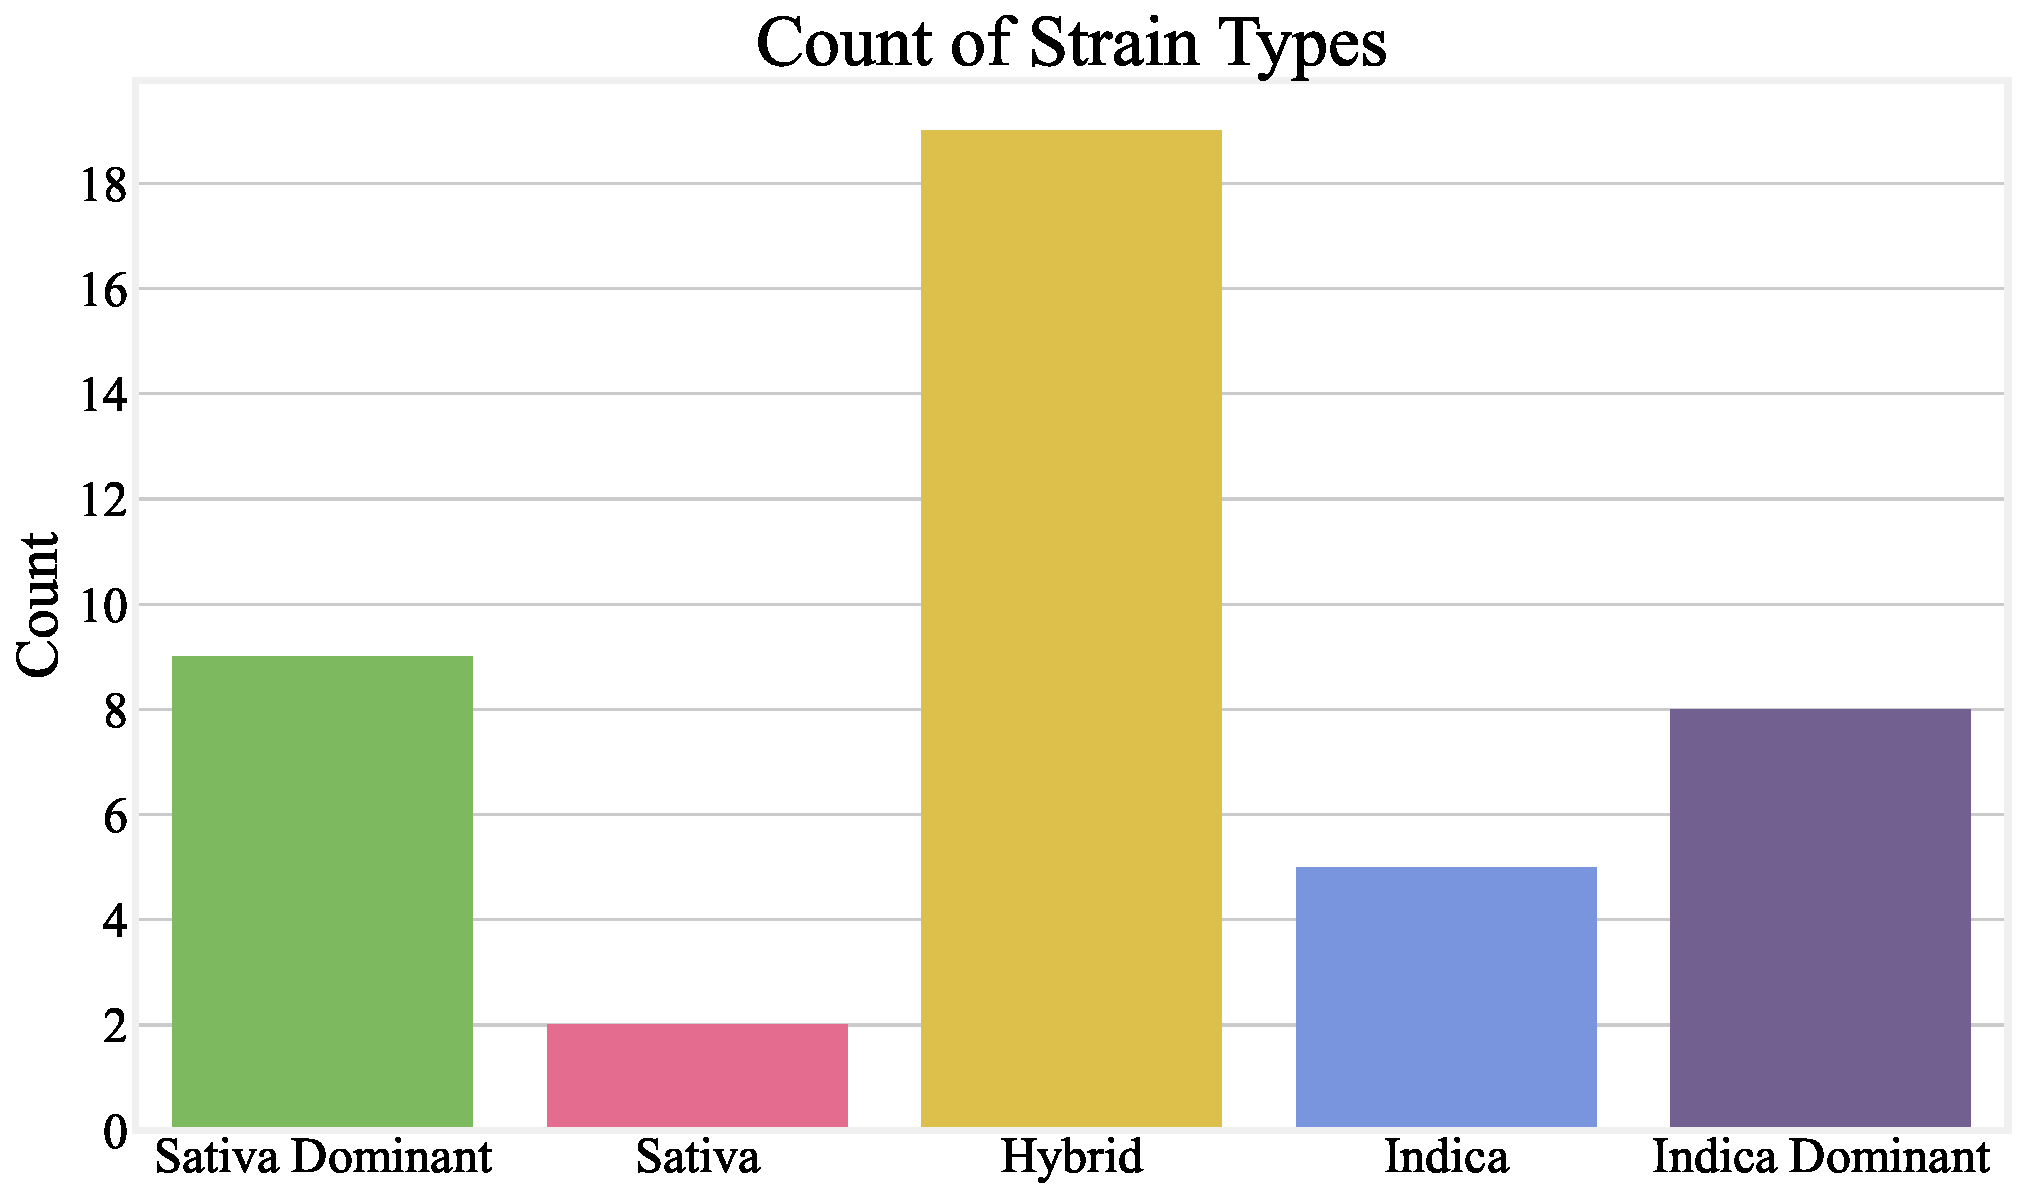
\includegraphics[width=0.75\linewidth]{figures/strain-types.pdf}

\end{multicols}

{\small
% Strain statistics
\begin{flushleft}
\subfile{stats/strains}
\end{flushleft}
}

{\small
% Summary table
\noindent Total Flow Gardens Data\\[0.25\baselineskip]
\subfile{stats/summary}
}


%---------------------------------%
% Reviews
%---------------------------------%
\newpage
\begin{multicols}{2}

\section*{Reviews}
\label{sec:Reviews}
\thispagestyle{regular}

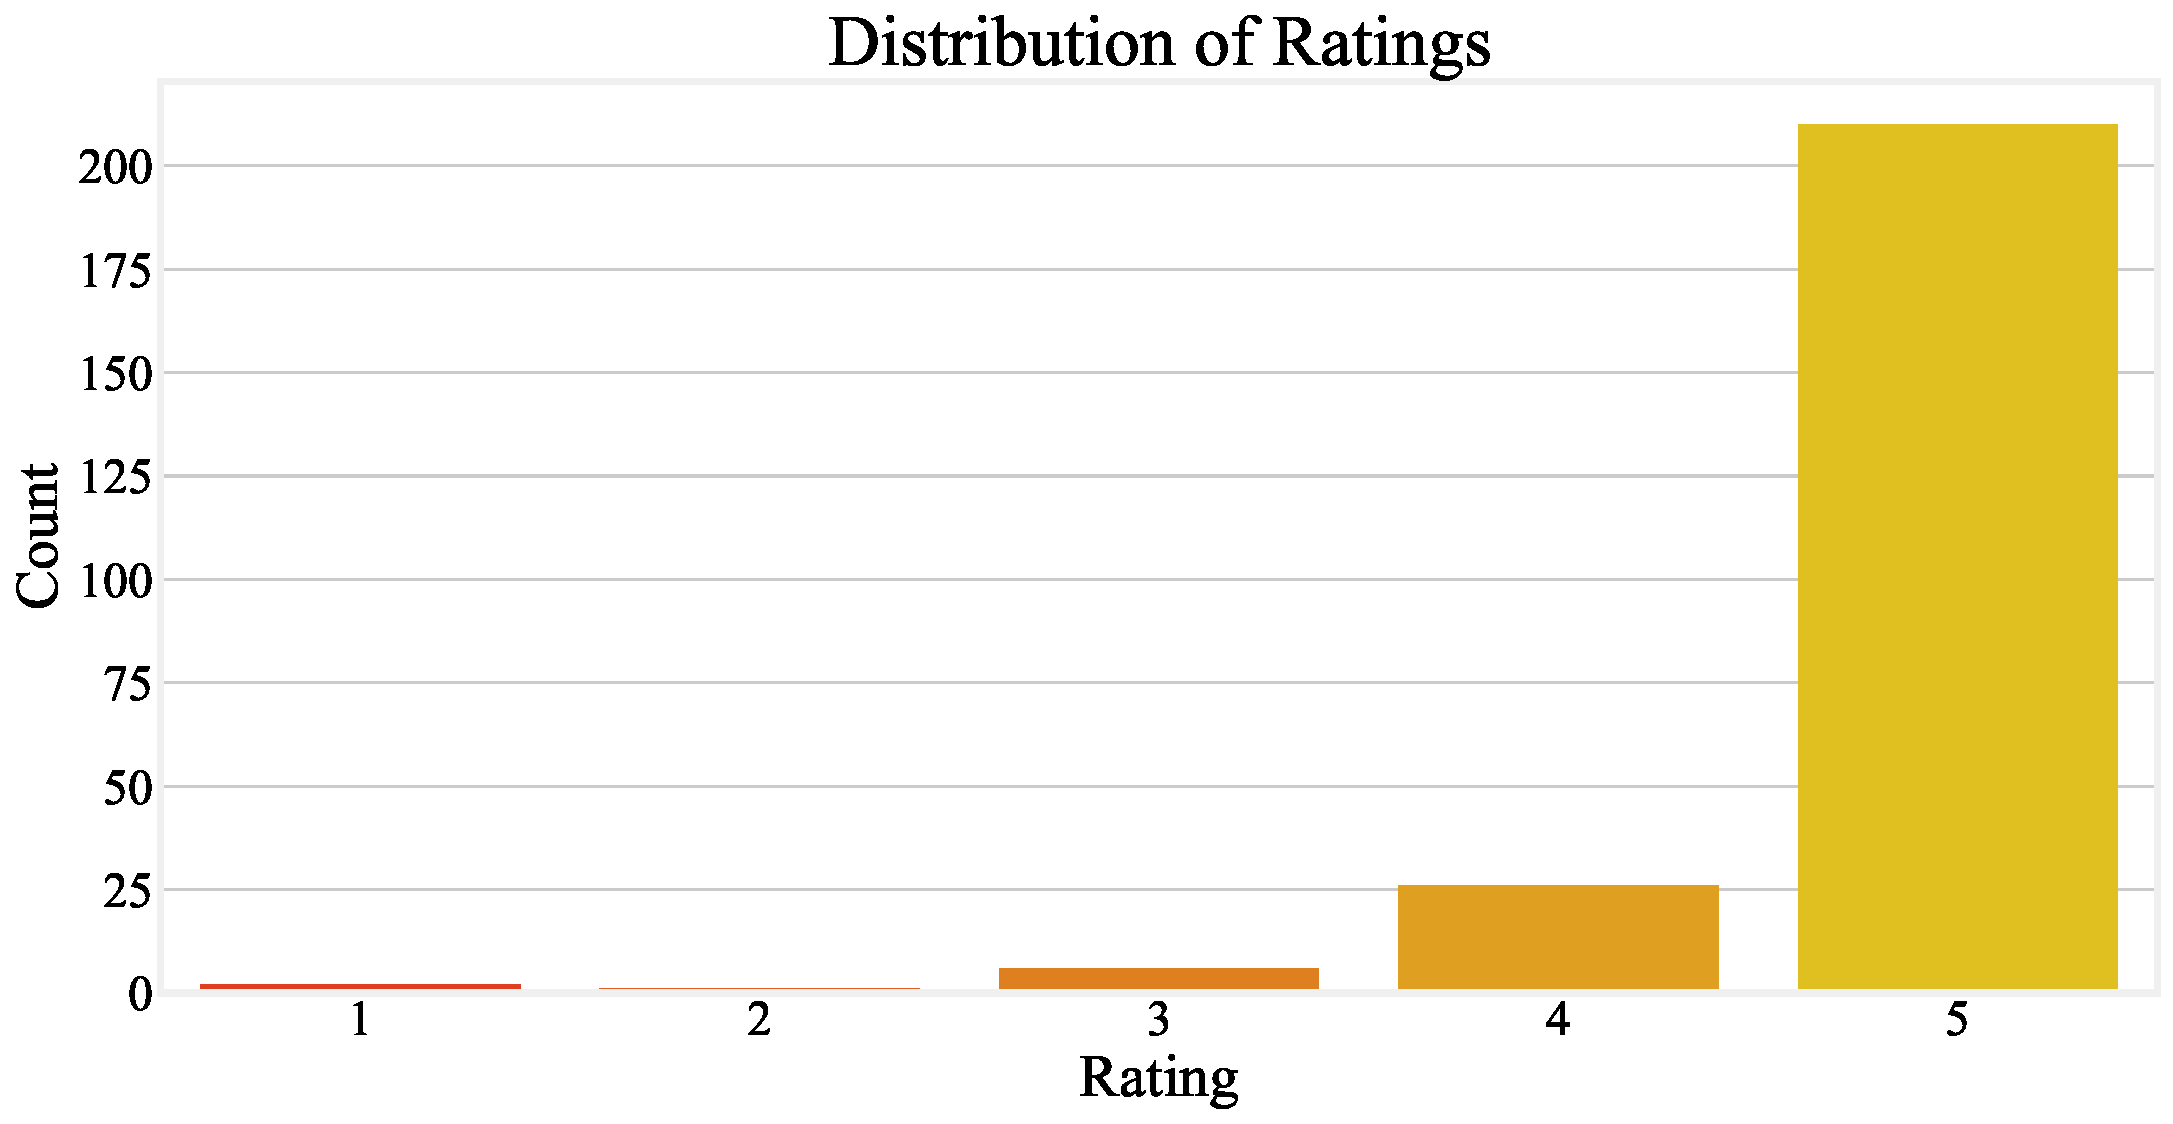
\includegraphics[width=\linewidth]{figures/ratings.pdf}

\vspace{1\baselineskip}

Reviews for strains were collected from Flow Gardens' website. Natural language processing (NLP) and the Vader Sentiment Intensity Analyzer (SIA) were used to measure the sentiment of each review. The average sentiment for each strain is depicted below, with lower values indicating lower sentiment and higher values indicating greater positivity.

\vspace{1\baselineskip}

% Strain sentiment figure.
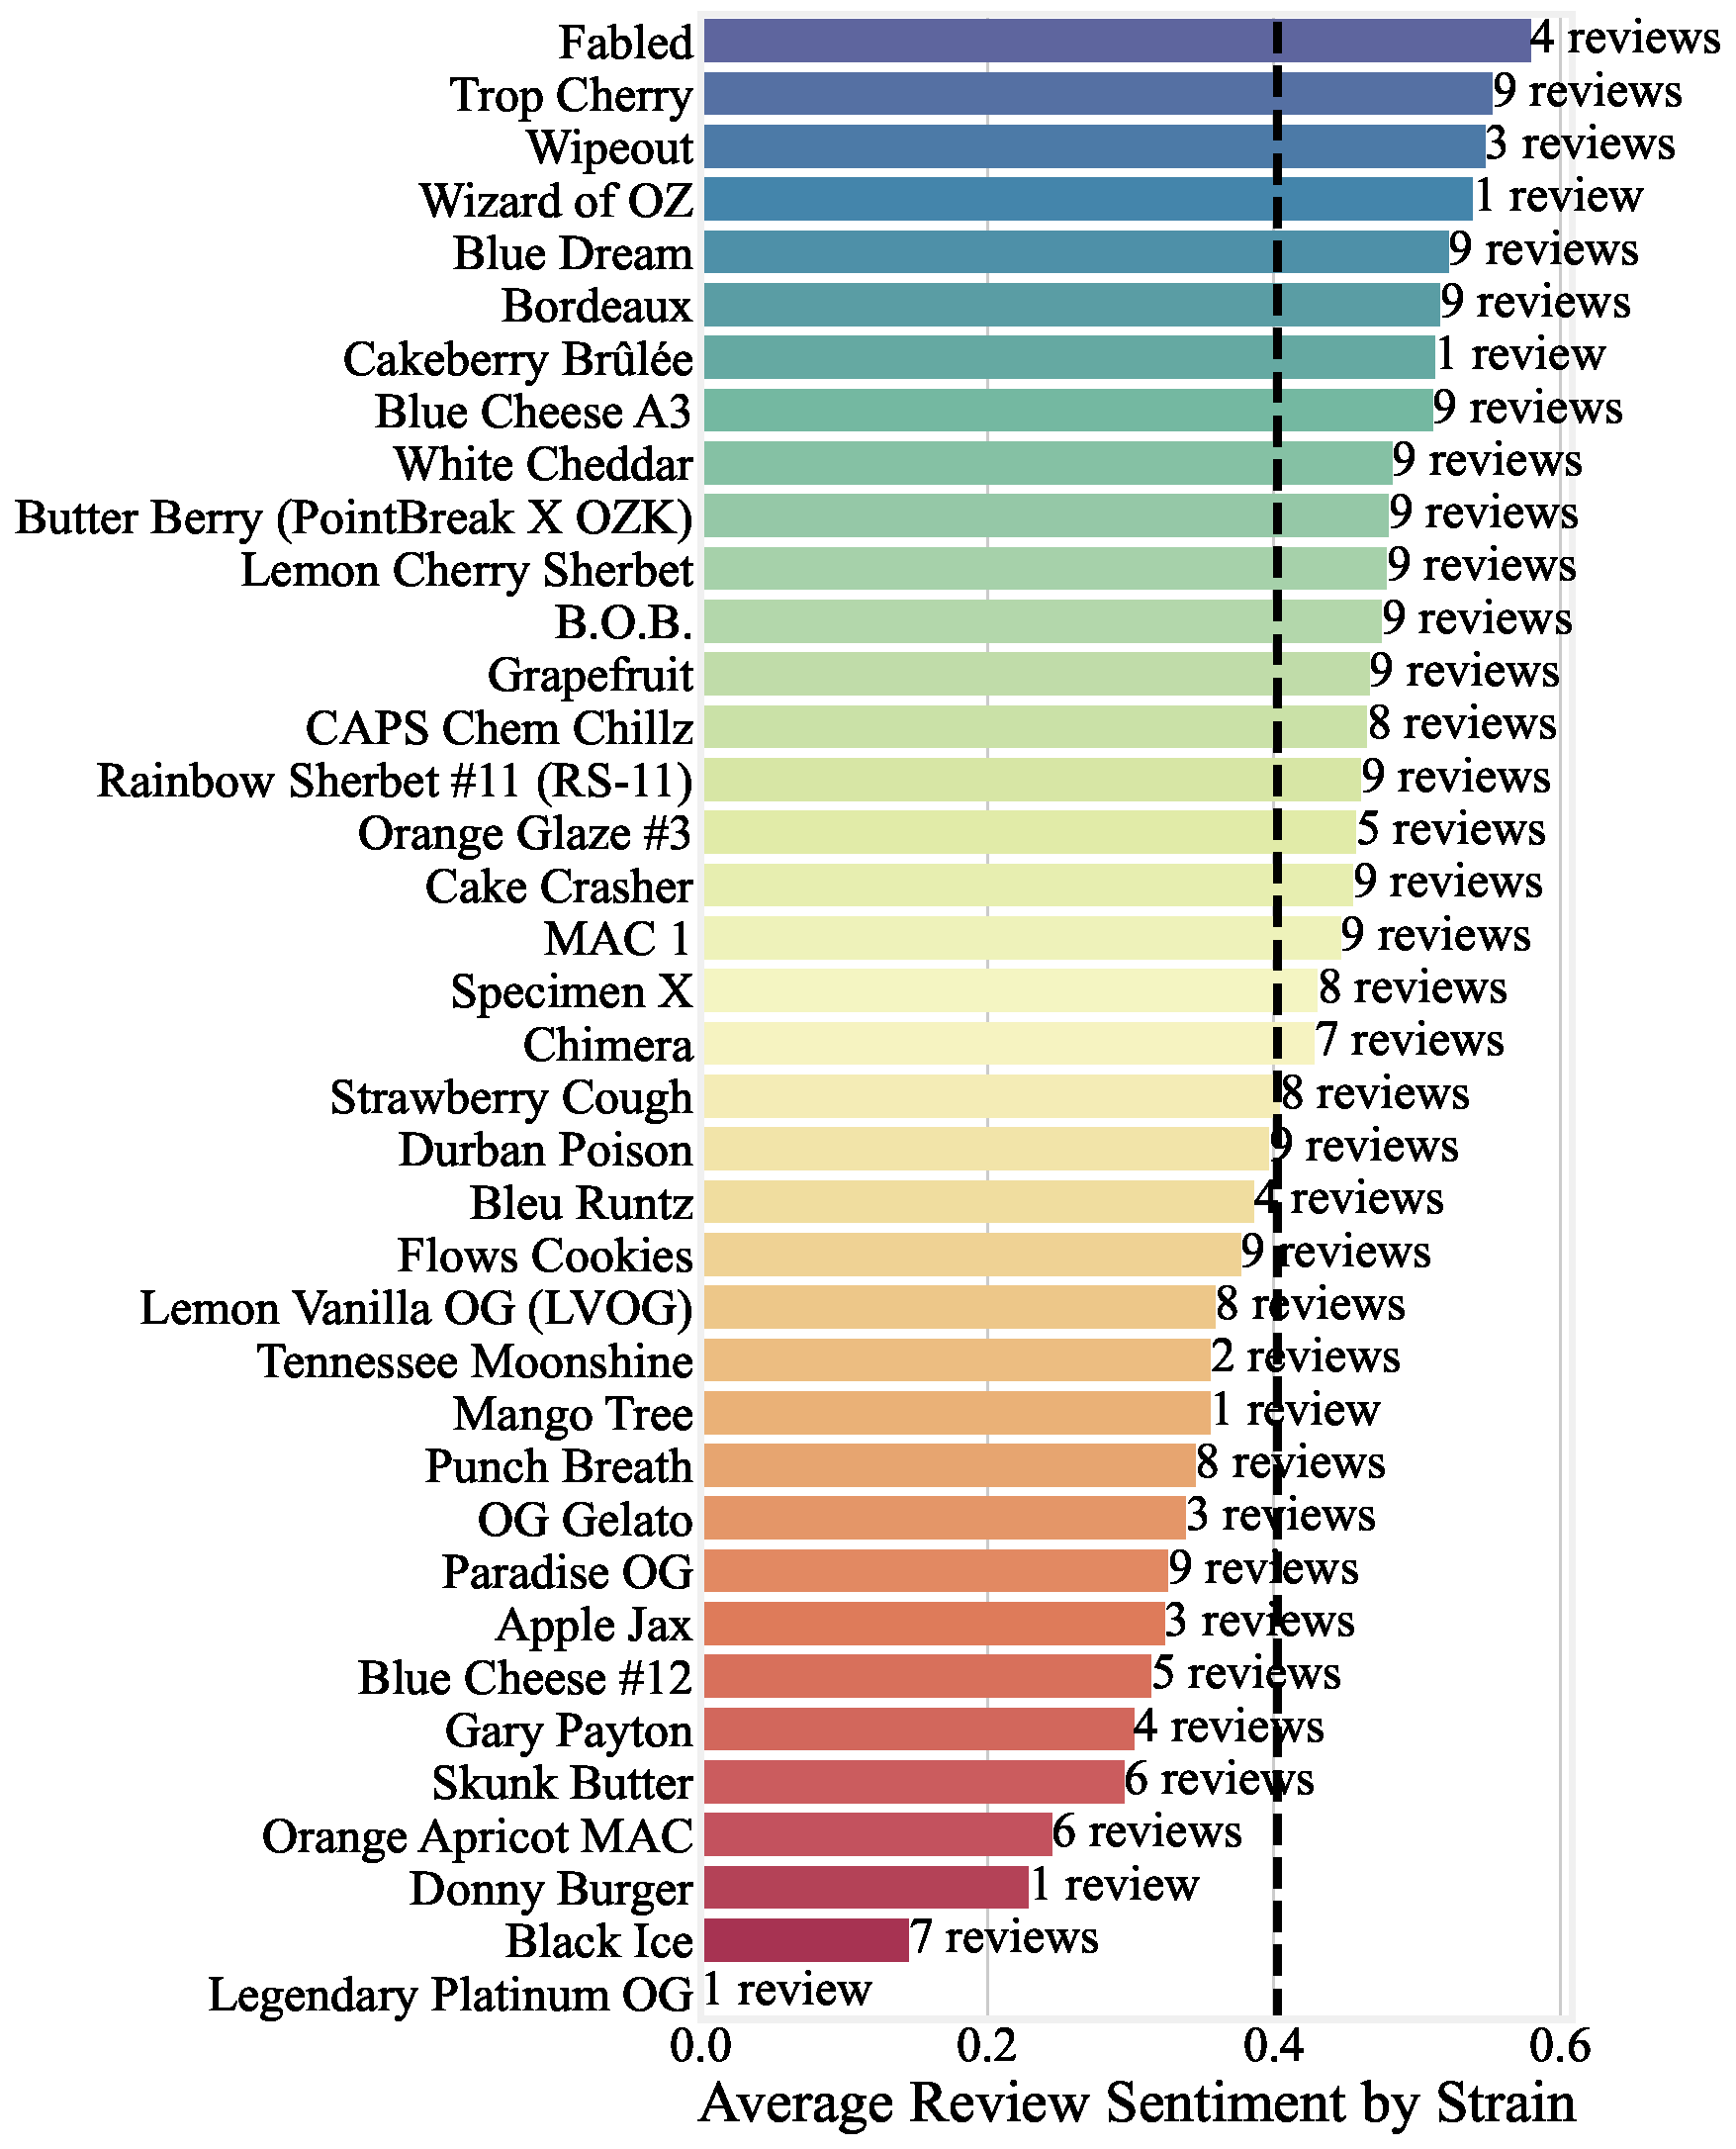
\includegraphics[width=\linewidth]{figures/strain-sentiment.pdf}

Effects and aromas were extracted using OpenAI's \texttt{gpt-4-0125-preview} model. The percentage of reviews that mention an effect or an aroma are shown in the following figures.

\vspace{1\baselineskip}

% Effects and aromas.
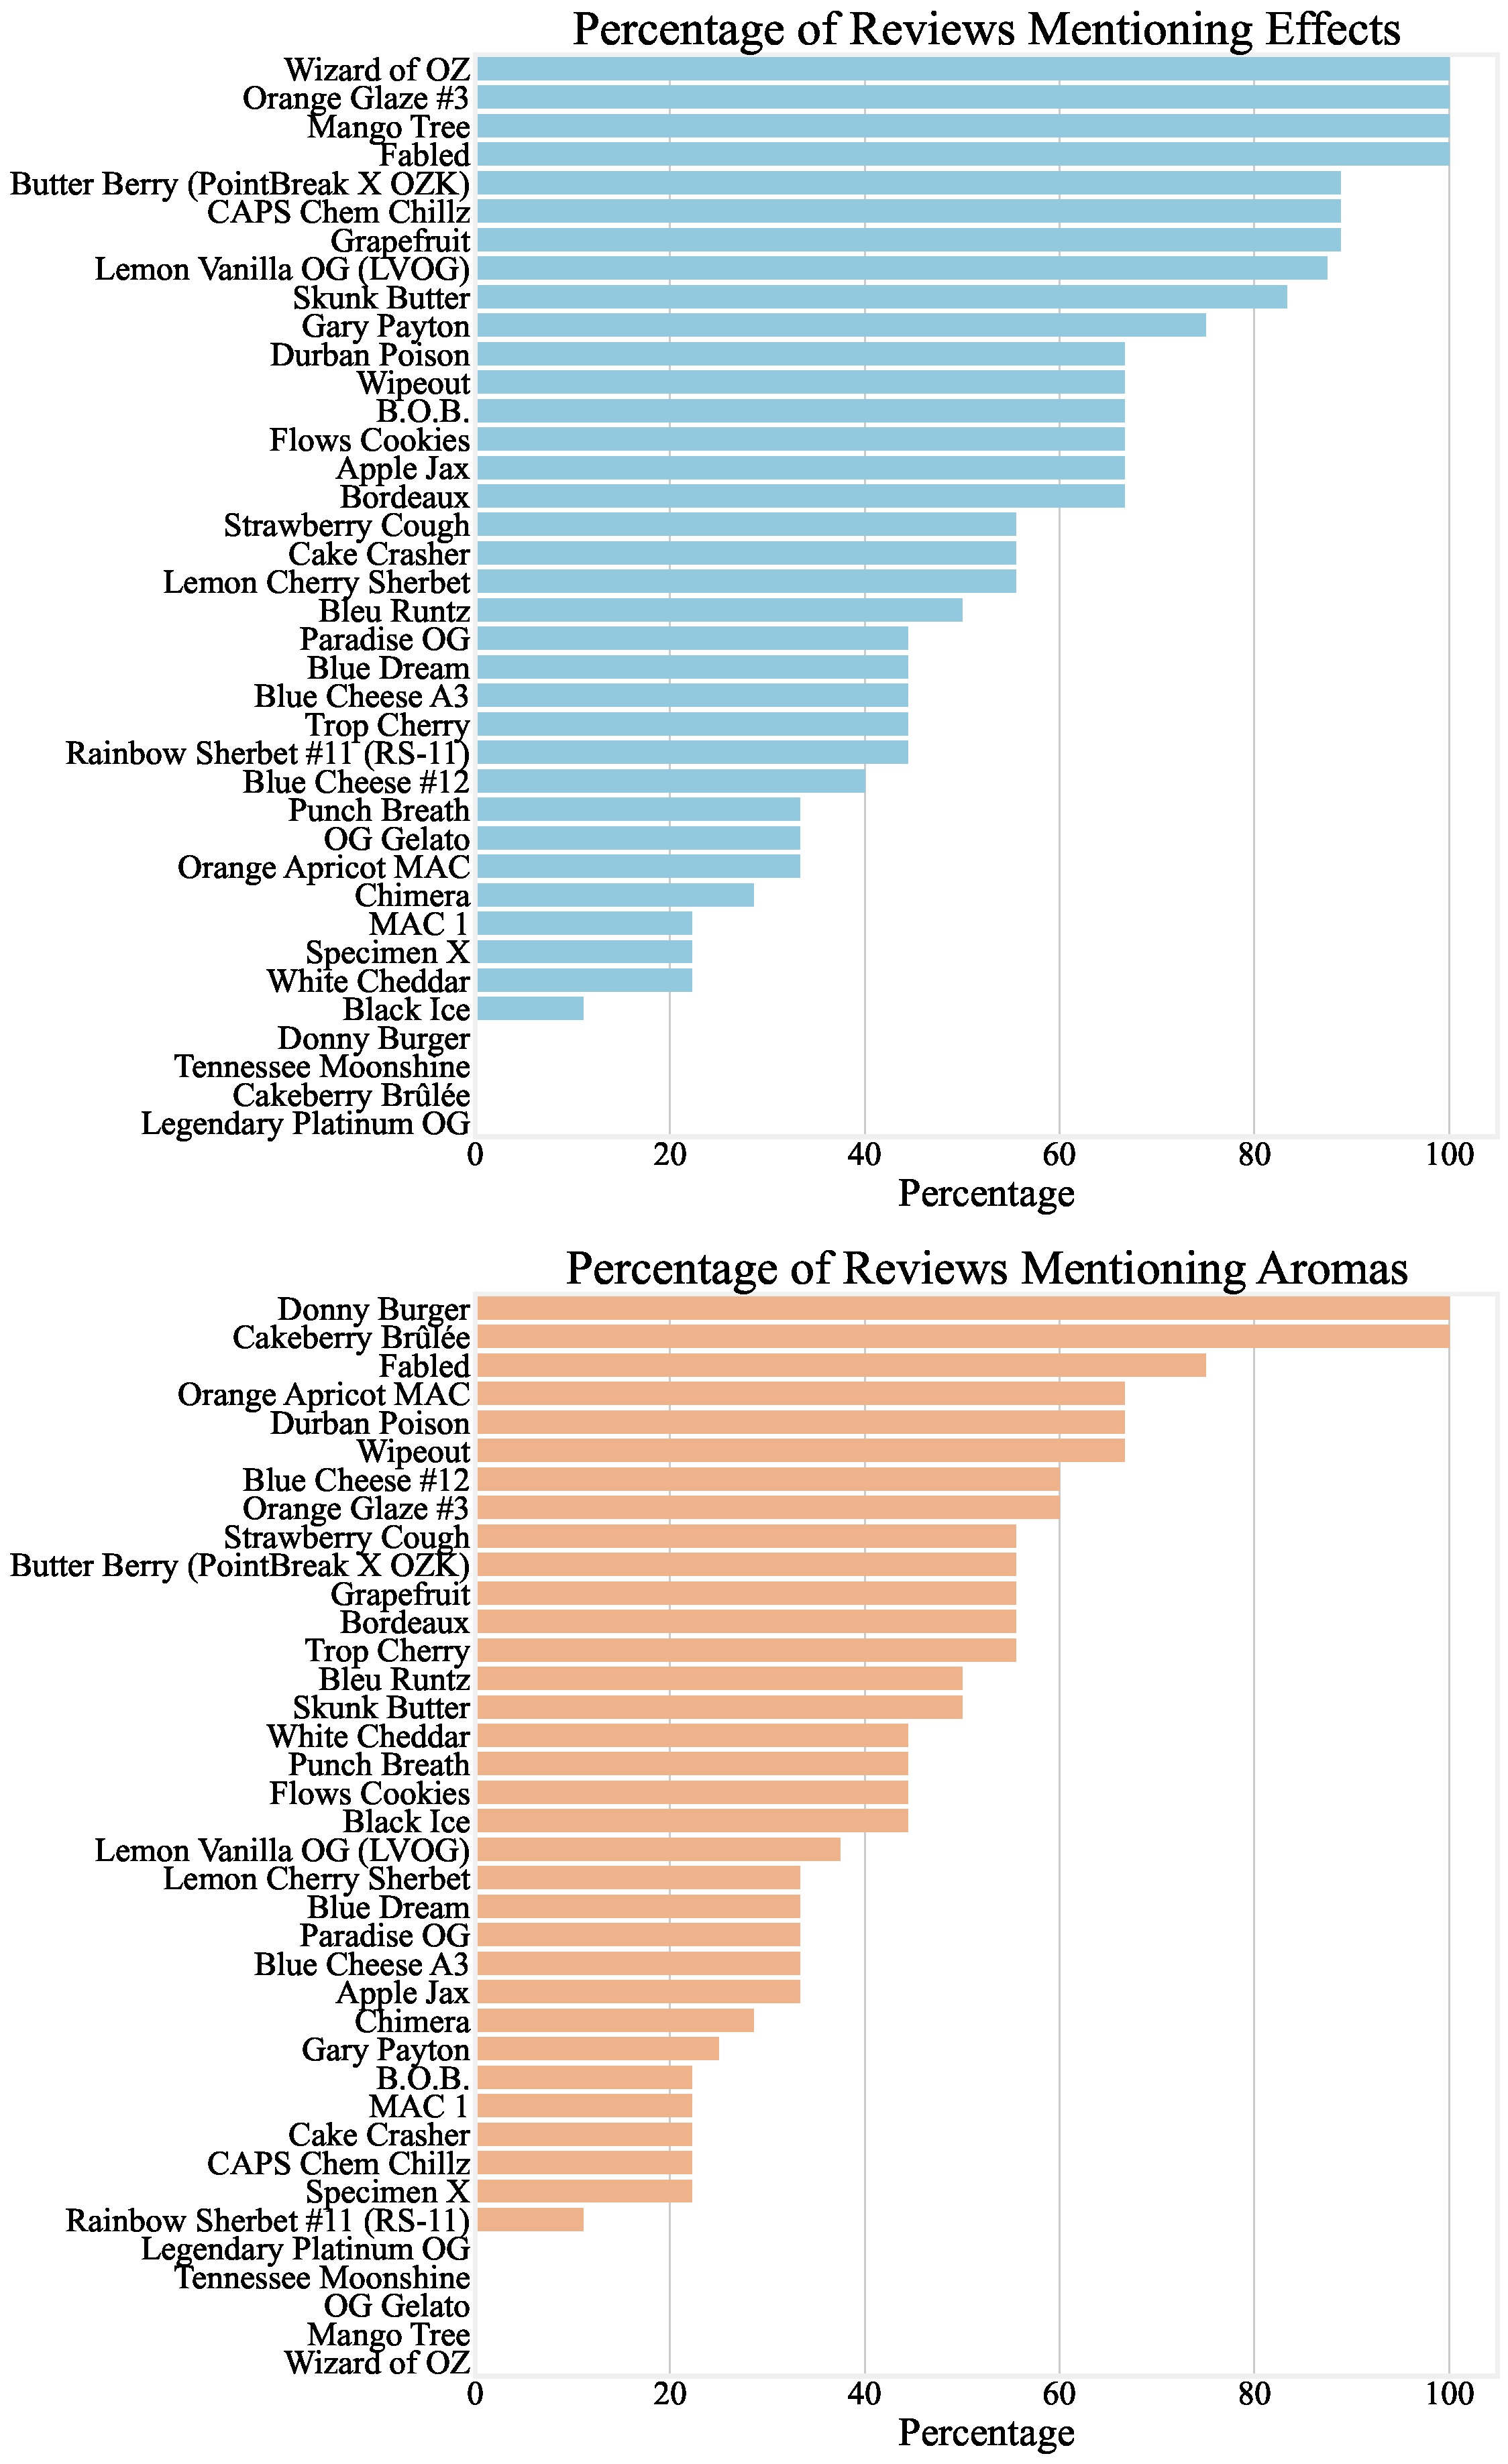
\includegraphics[width=\linewidth]{figures/aromas-effects.pdf}

\vspace{1\baselineskip}

Finally, we look at the reviews that mention {\itshape Sativa} or {\itshape Indica}, corresponding strain names, and designated strain types. This can give an idea of how well users are utilizing current classifications.

\vspace{0.5\baselineskip}

{\scriptsize

\vspace{1\baselineskip}

\subfile{stats/sativa-mentions}

\vspace{1\baselineskip}

\subfile{stats/indica-mentions}
}


%---------------------------------%
% Images
%---------------------------------%
\newpage
\section*{Strain Images}
\label{sec:Strain Images}

Images for each strain were analyzed for their {\itshape colorfulness} and {\itshape purpleness}. These are simply rudimentary measures of color to help quantify each strain.

\vspace{1\baselineskip}

% Colorfulness
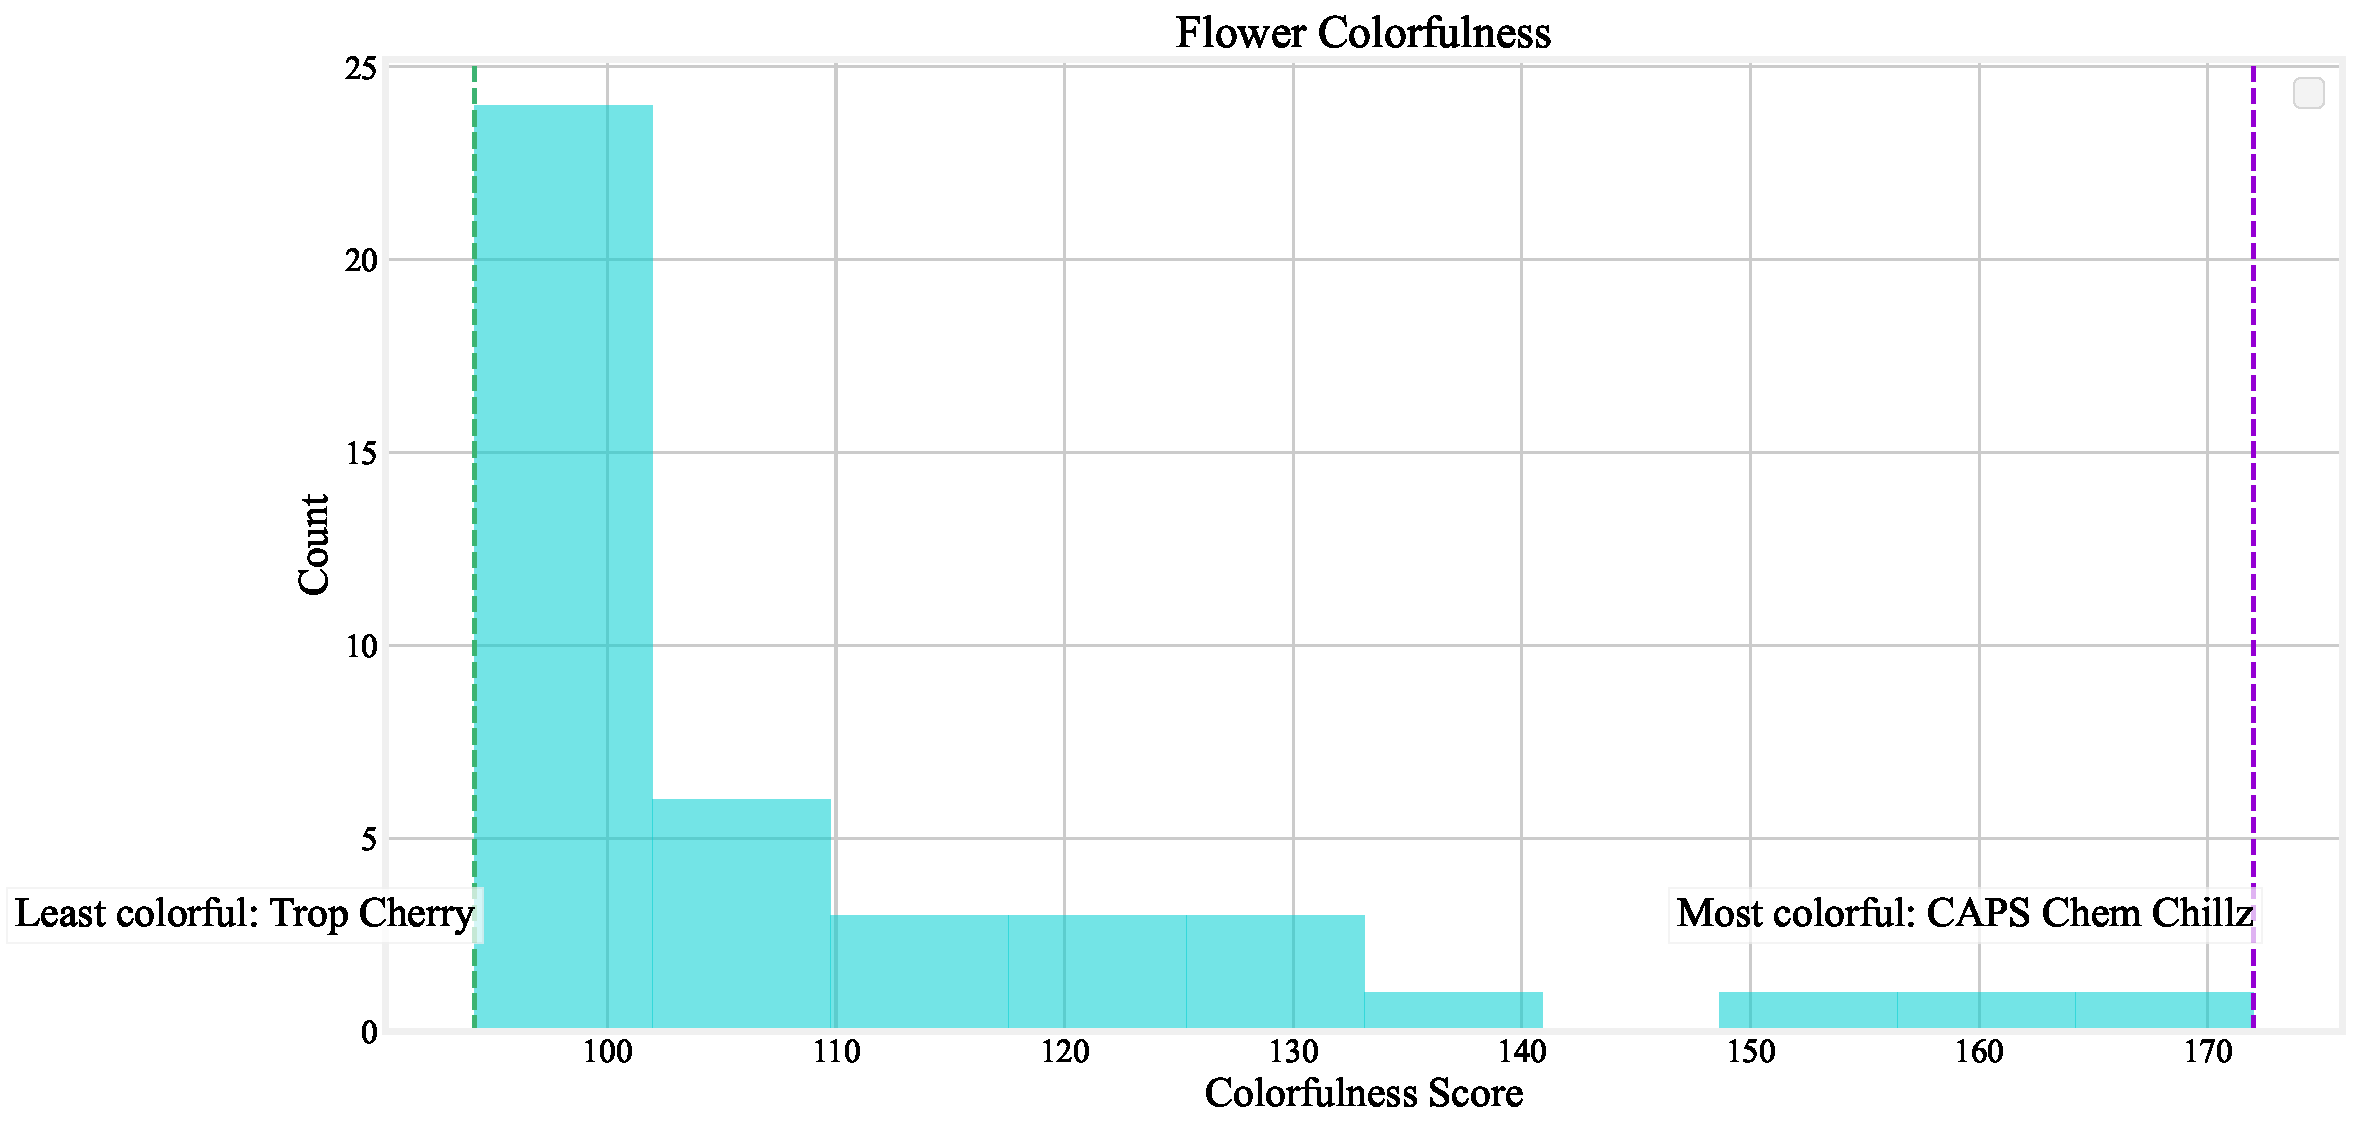
\includegraphics[width=\linewidth]{figures/colorfulness.pdf}

\vspace{1\baselineskip}

The measure of {\itshape purpleness} can be used to identify strains that people would recognize as purple. Alternatively, the inverse of {\itshape purplenss} is {\itshape greenness}, which could be a desirable trait in its own right.

\vspace{1\baselineskip}

% Purpleness
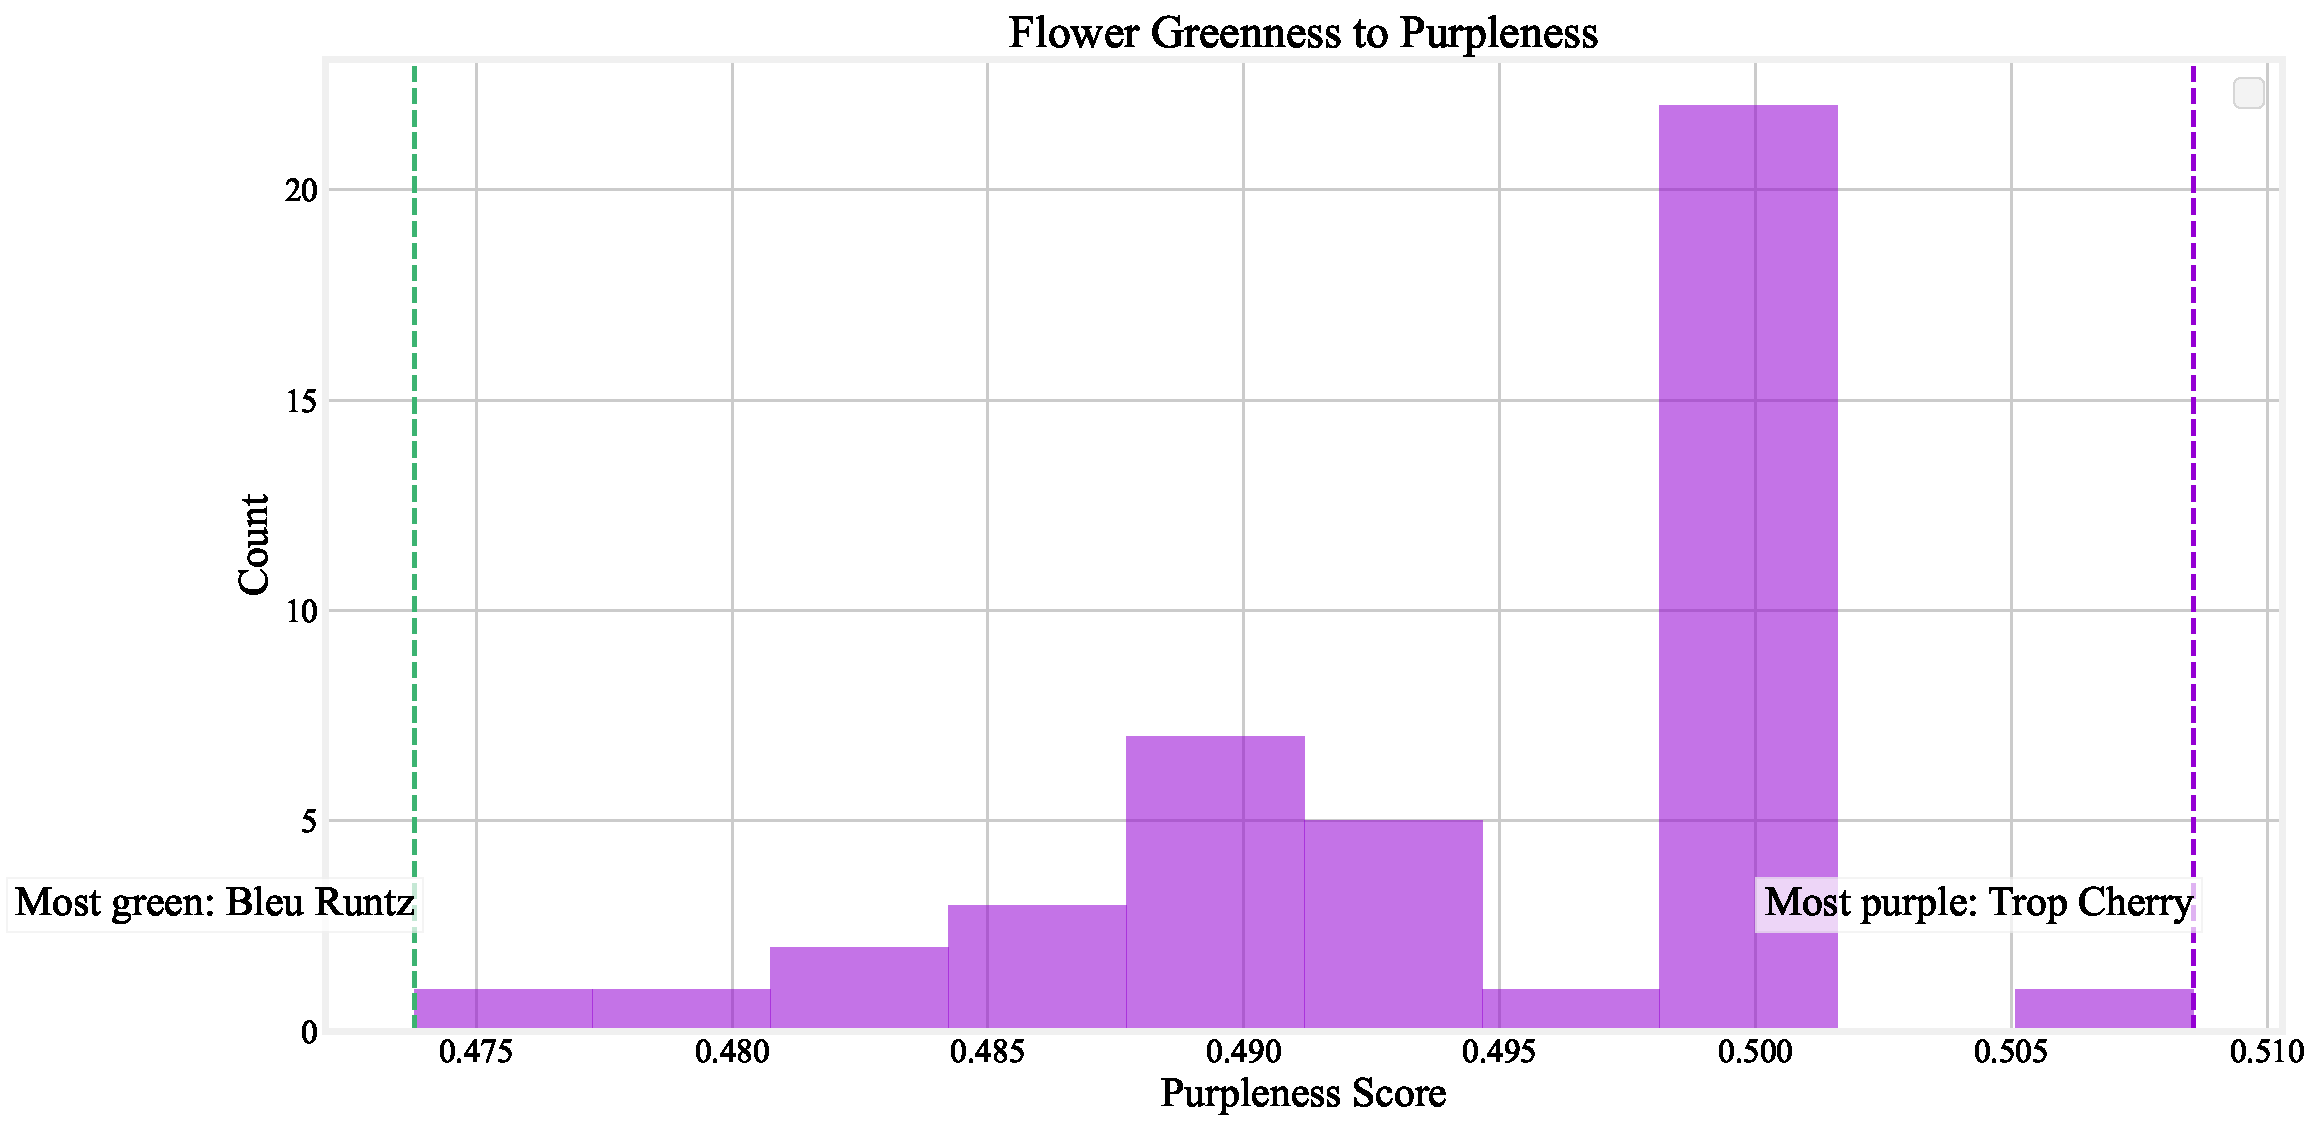
\includegraphics[width=\linewidth]{figures/purpleness.pdf}

% TODO: Table of colorfulness and purpleness.
{\scriptsize
\vspace{1\baselineskip}
\subfile{stats/colors}
}


%---------------------------------%
% Chemical Analysis
%---------------------------------%
\newpage
\section*{Chemical Analysis}
\label{sec:Chemical Analysis}
\thispagestyle{regular}

First, we examine THCA, $\Delta$-9 THC, and CBD concentrations. We then look at the total cannabinoids and the total terpenes. Next, CBGA and other minor cannabinoids are visualized. Then, ratios of dominant terpenes are examined. We also use the Shannon Diversity Index to quantify the diversity of terpenes and cannabinoids found in each strain. Finally, PCA scores are calculated using observed dominant terpenes to create clusters of chemically similar strains.

\vspace{1\baselineskip}

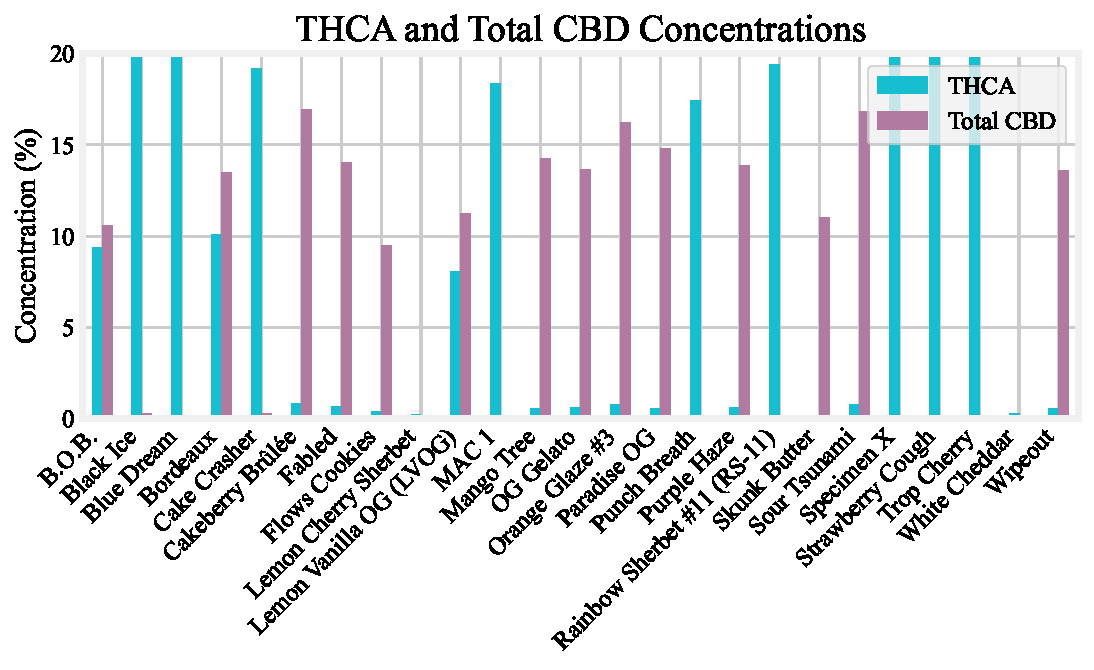
\includegraphics[width=0.95\linewidth]{figures/thca-cbd.pdf}

\vspace{1\baselineskip}

% Cannabinoid and terpene diversity bar plot.
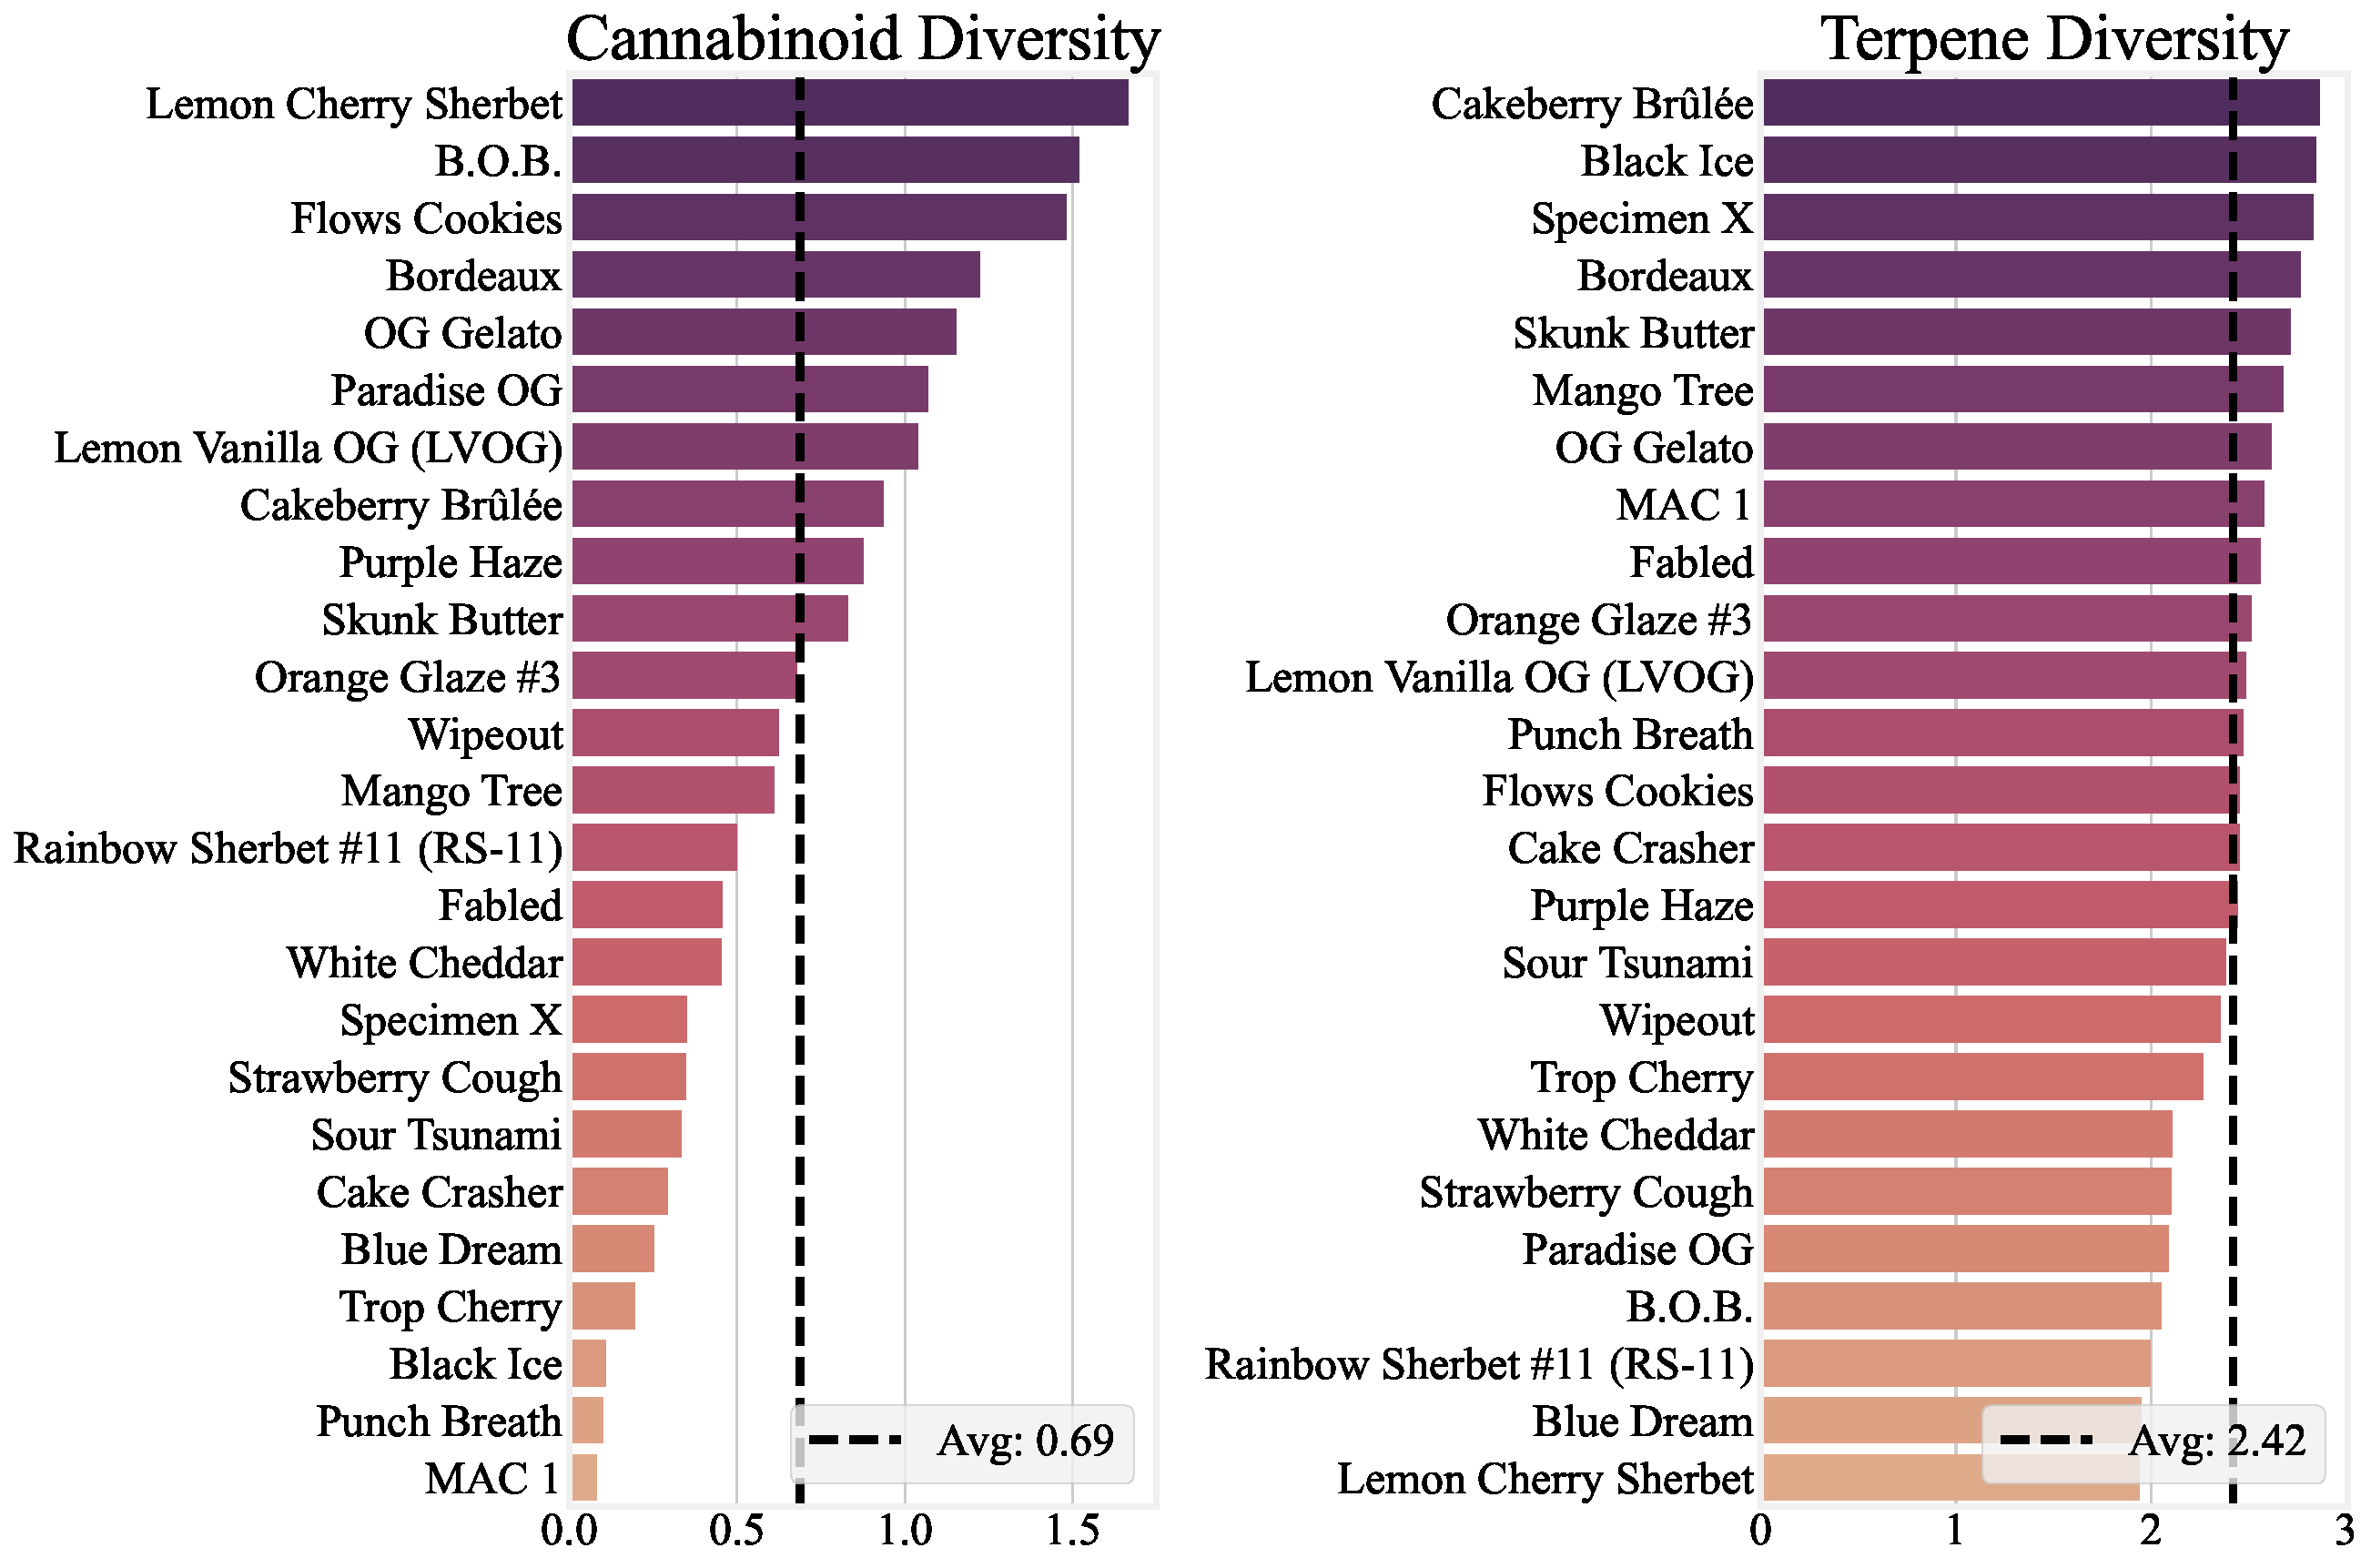
\includegraphics[width=0.95\linewidth]{figures/diversity.pdf}

\vspace{2\baselineskip}

% Chemical diversity scatterplot
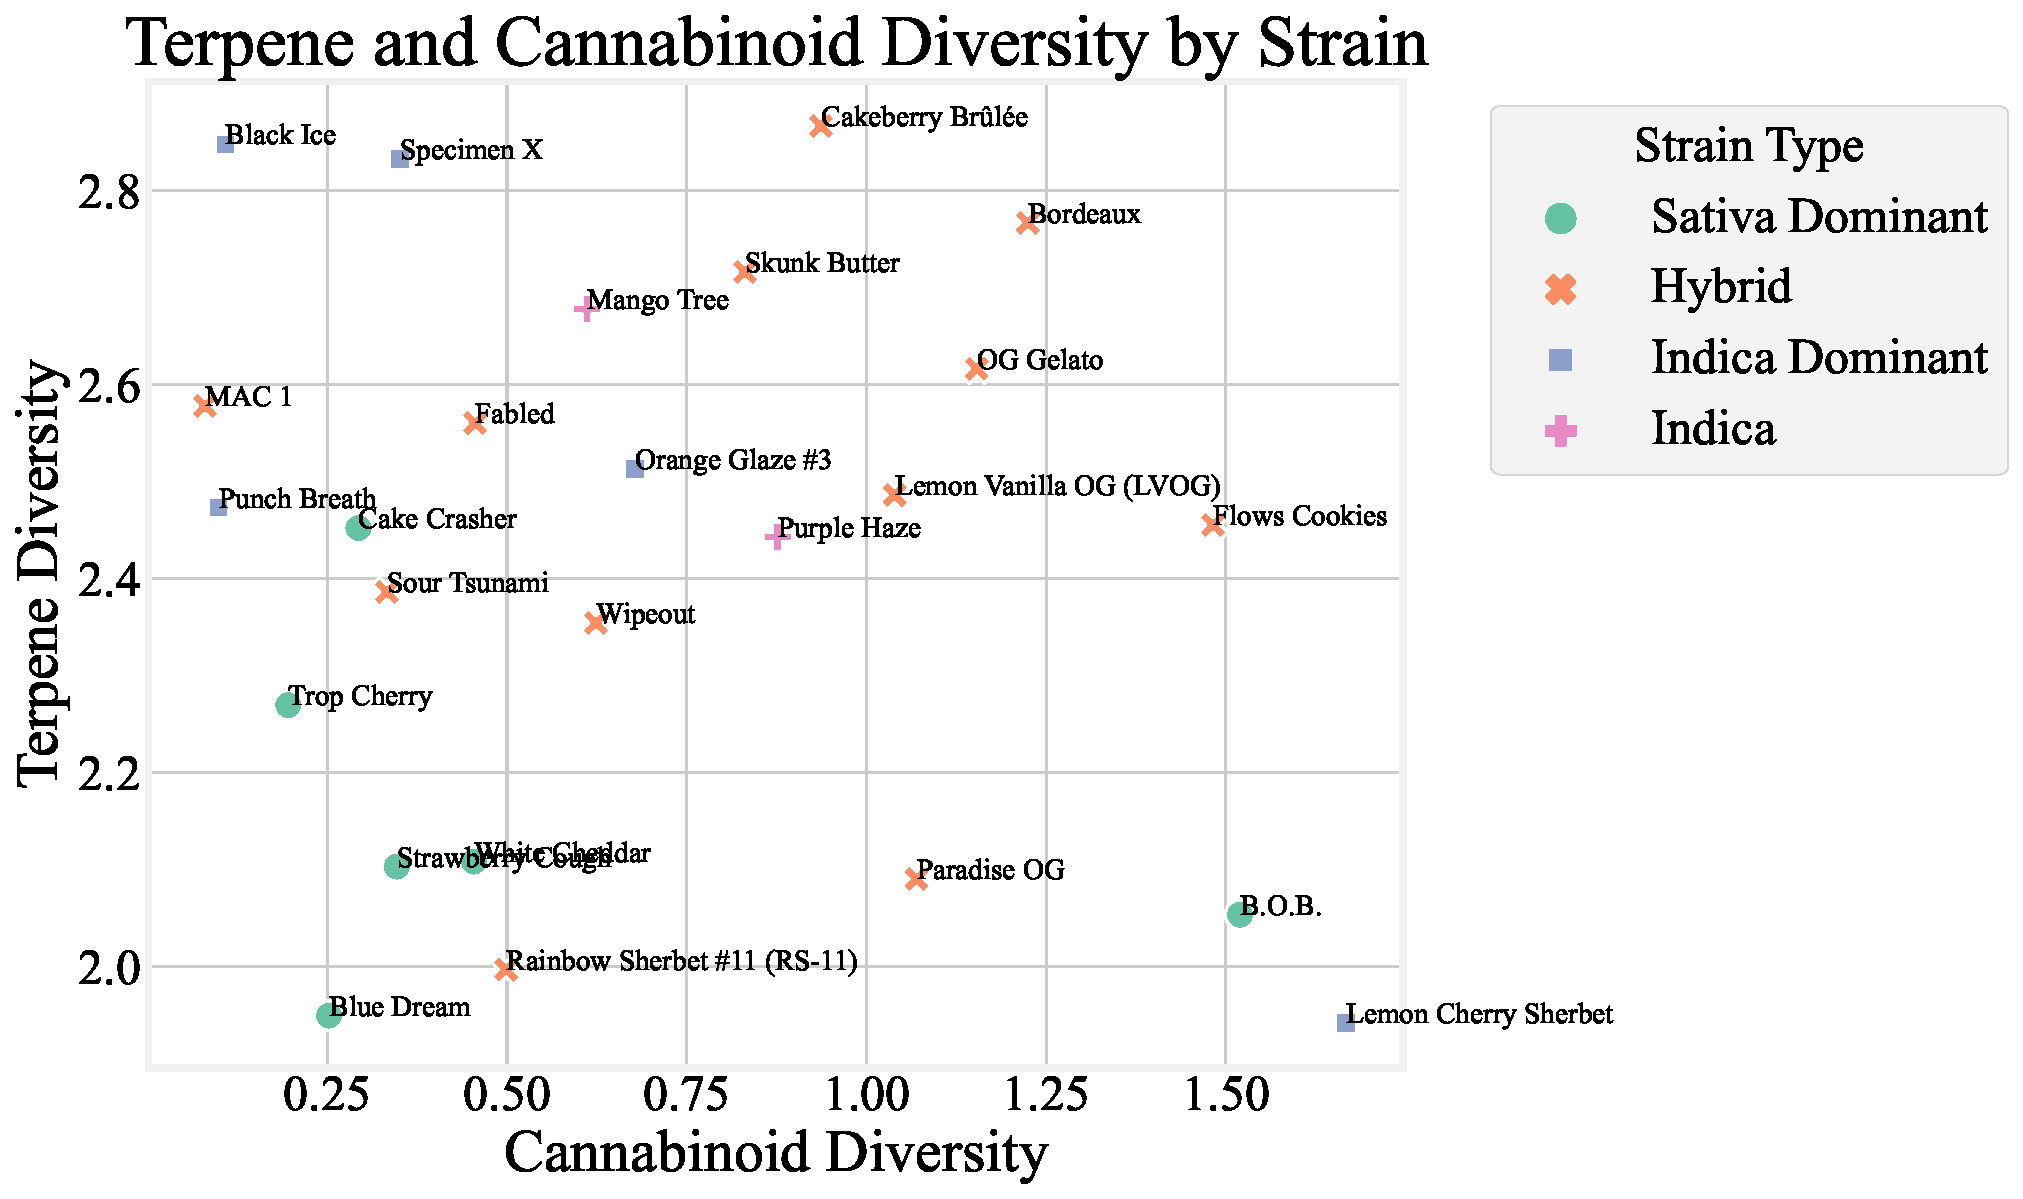
\includegraphics[width=0.95\linewidth]{figures/diversity-scatterplot.pdf}

\vspace{2\baselineskip}

% Compounds
{\tiny
\vspace{1\baselineskip}
\subfile{stats/compounds}
}

% Dominant terpenes.
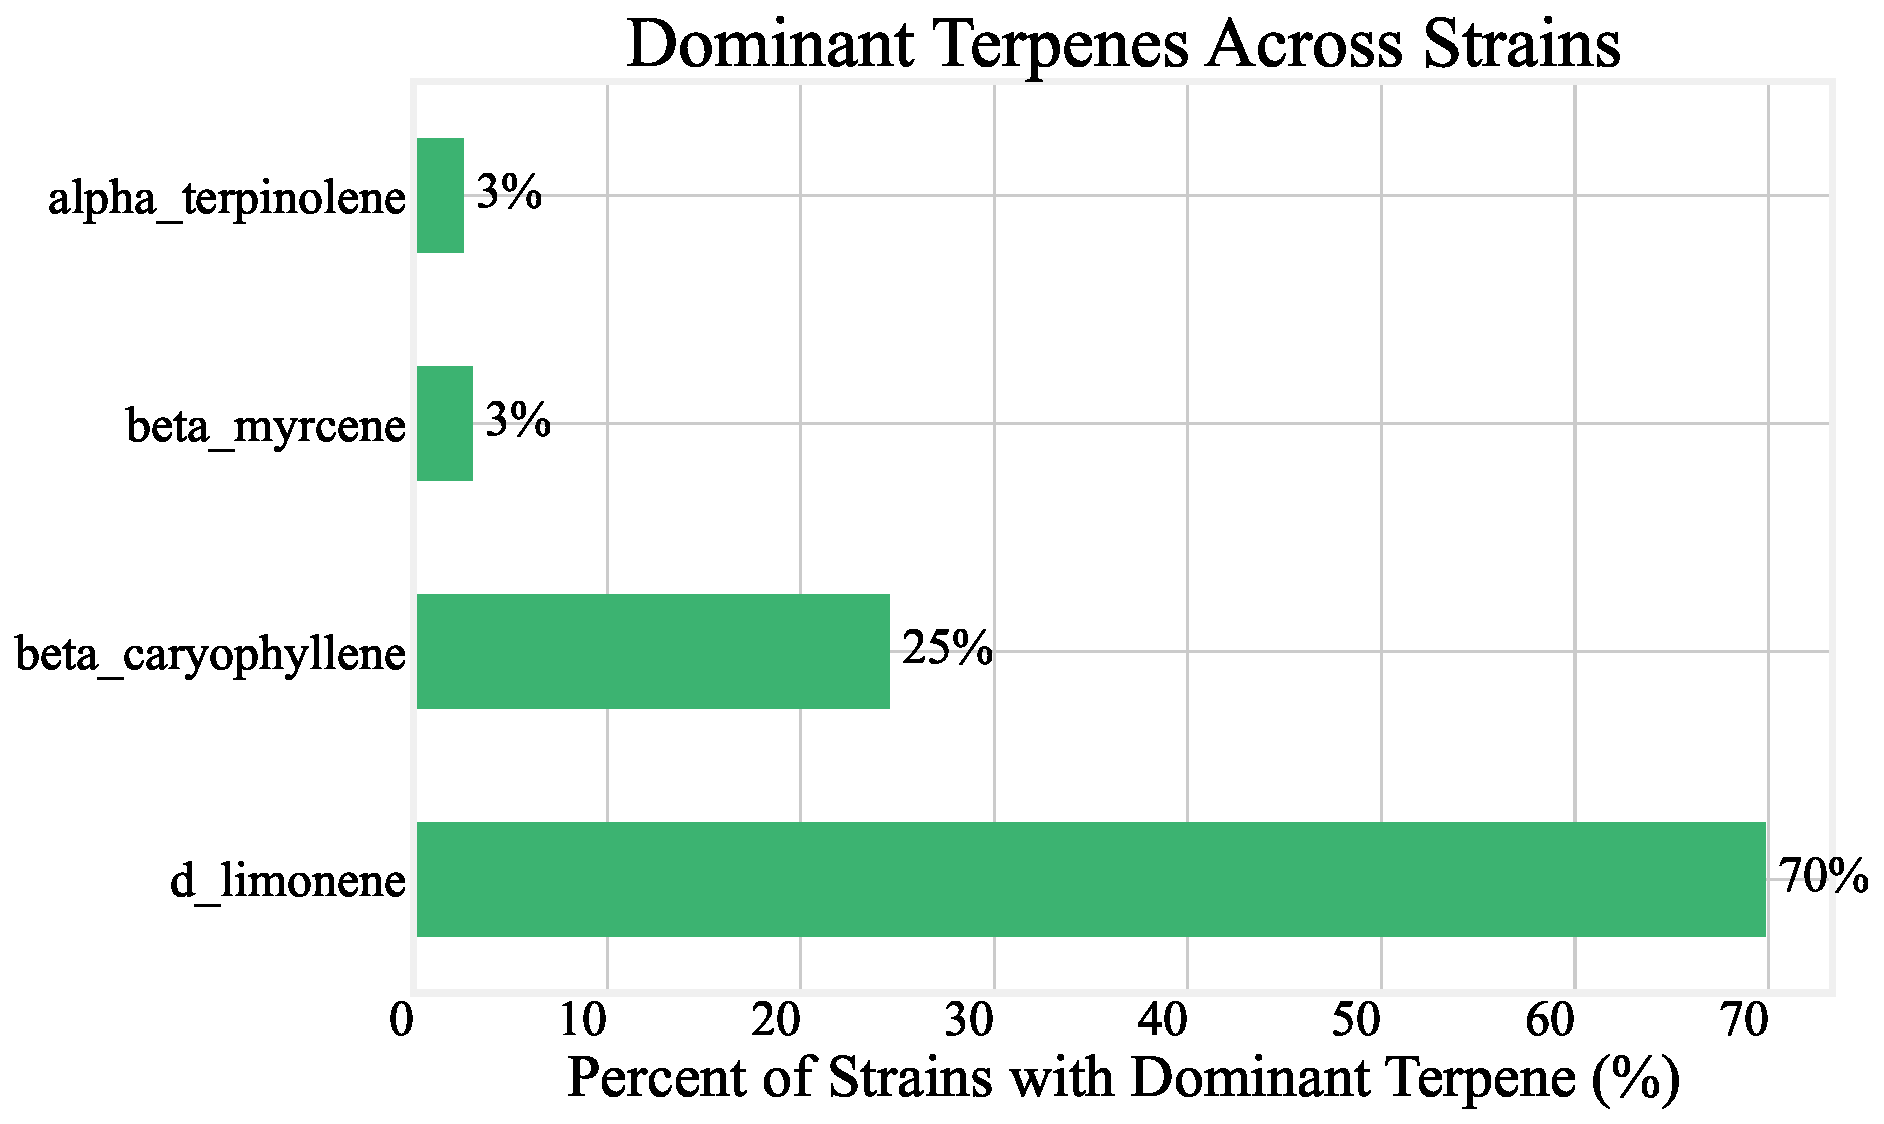
\includegraphics[width=0.95\linewidth]{figures/dominant-terpenes.pdf}


%% Optional: Average cannabinoid profile.
%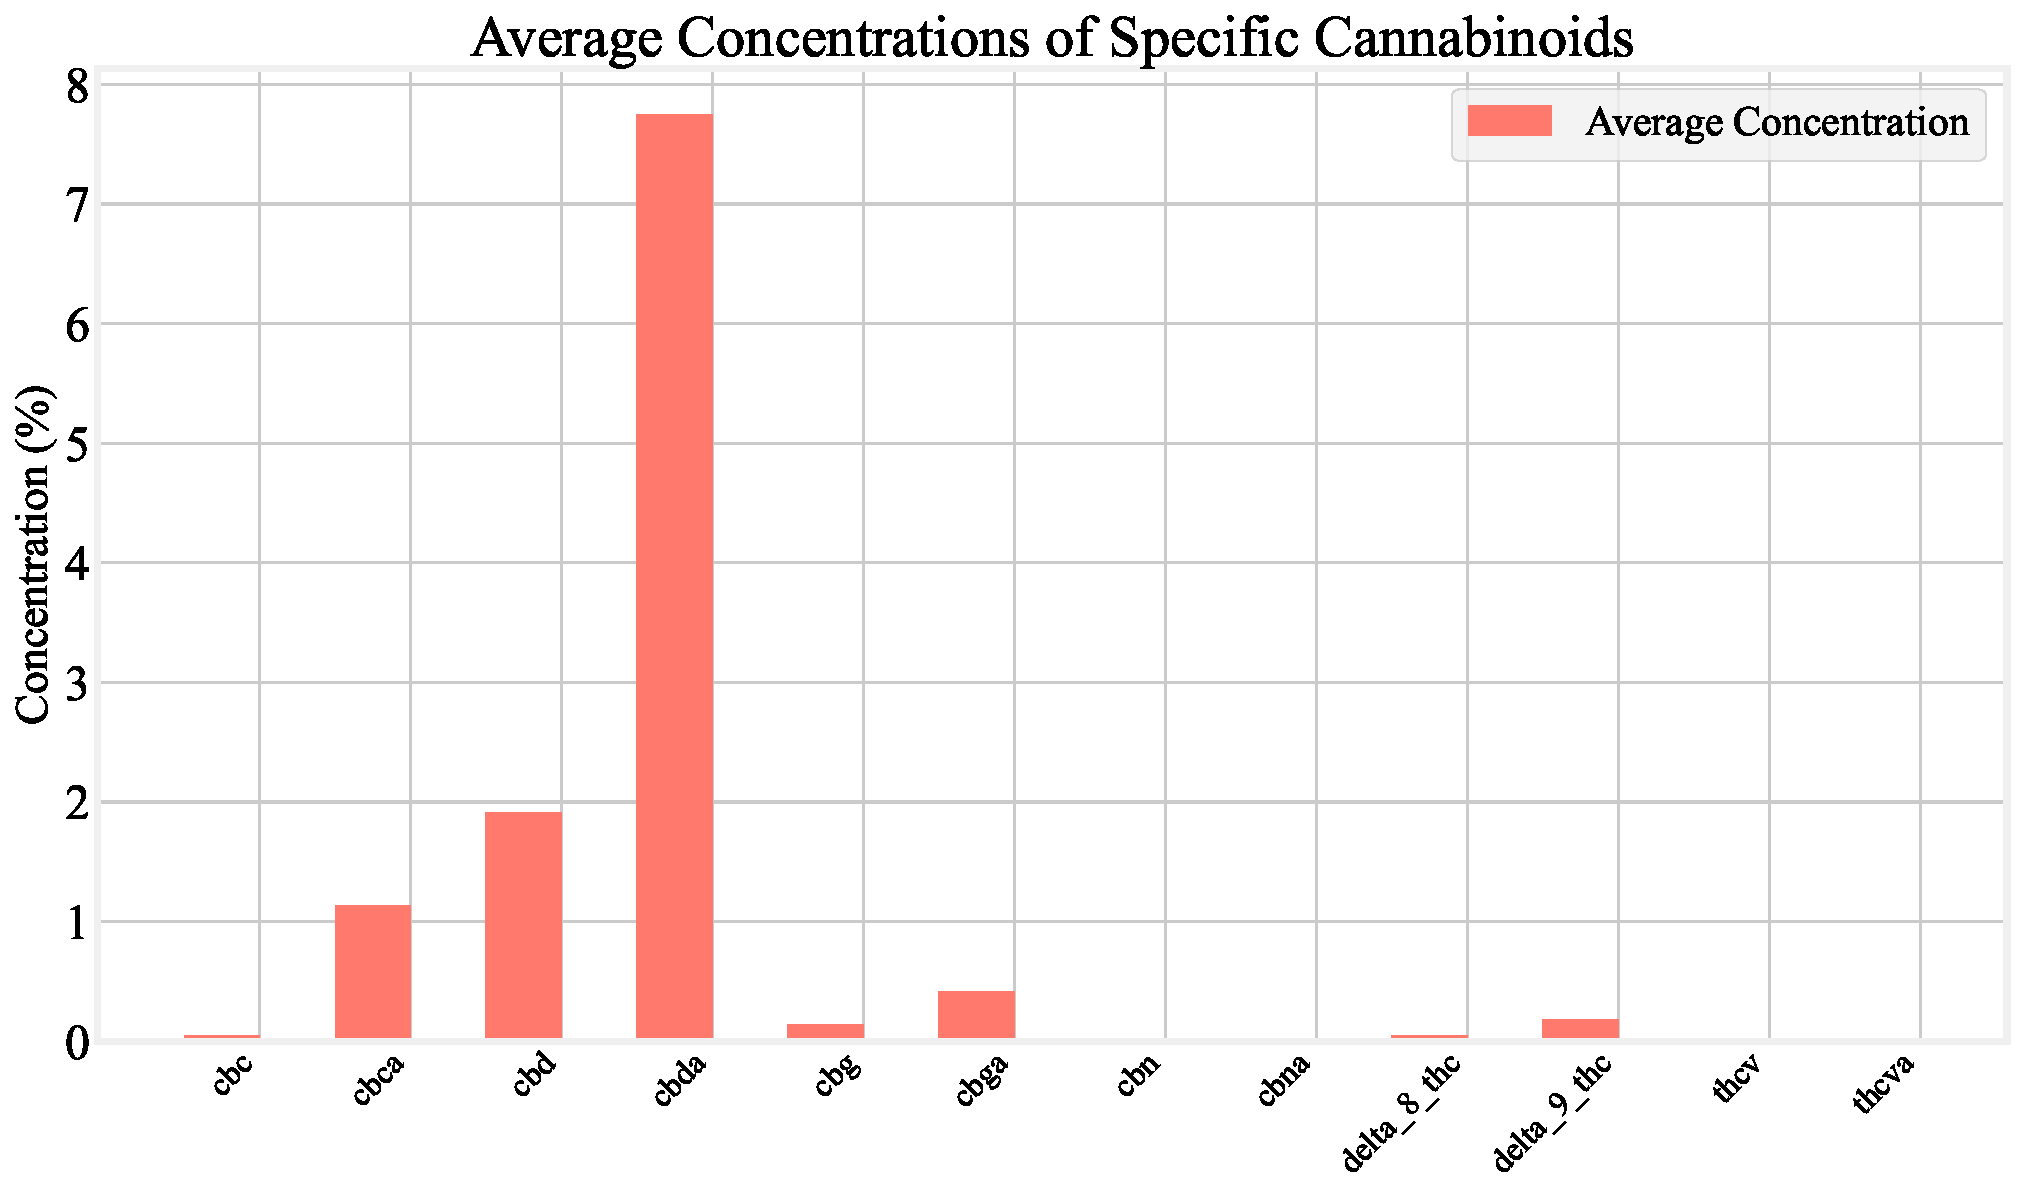
\includegraphics[width=0.95\linewidth]{figures/cannabinoids.pdf}
%
%
%% Optional: Average terpene profile.
%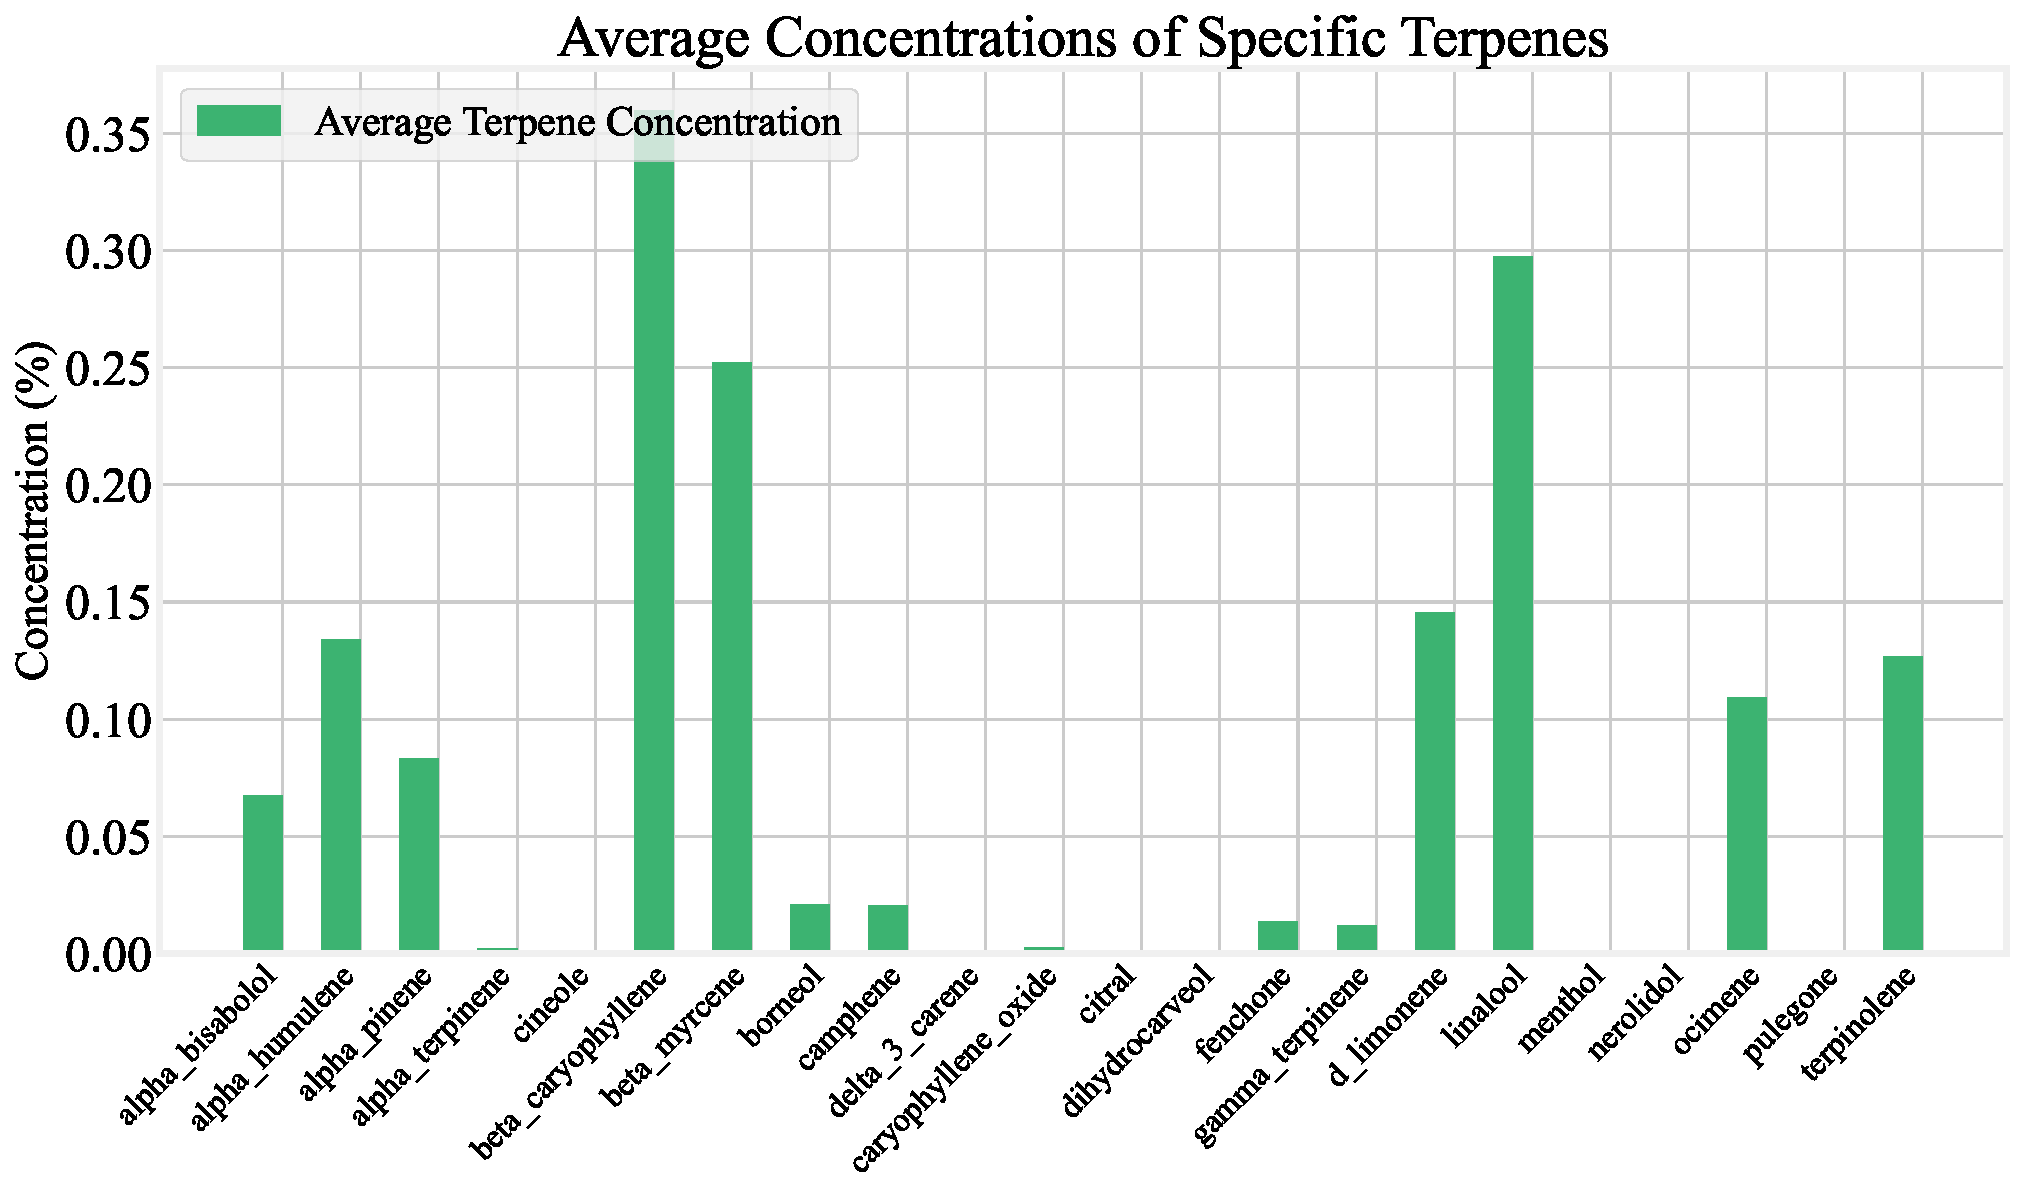
\includegraphics[width=0.95\linewidth]{figures/terpenes.pdf}


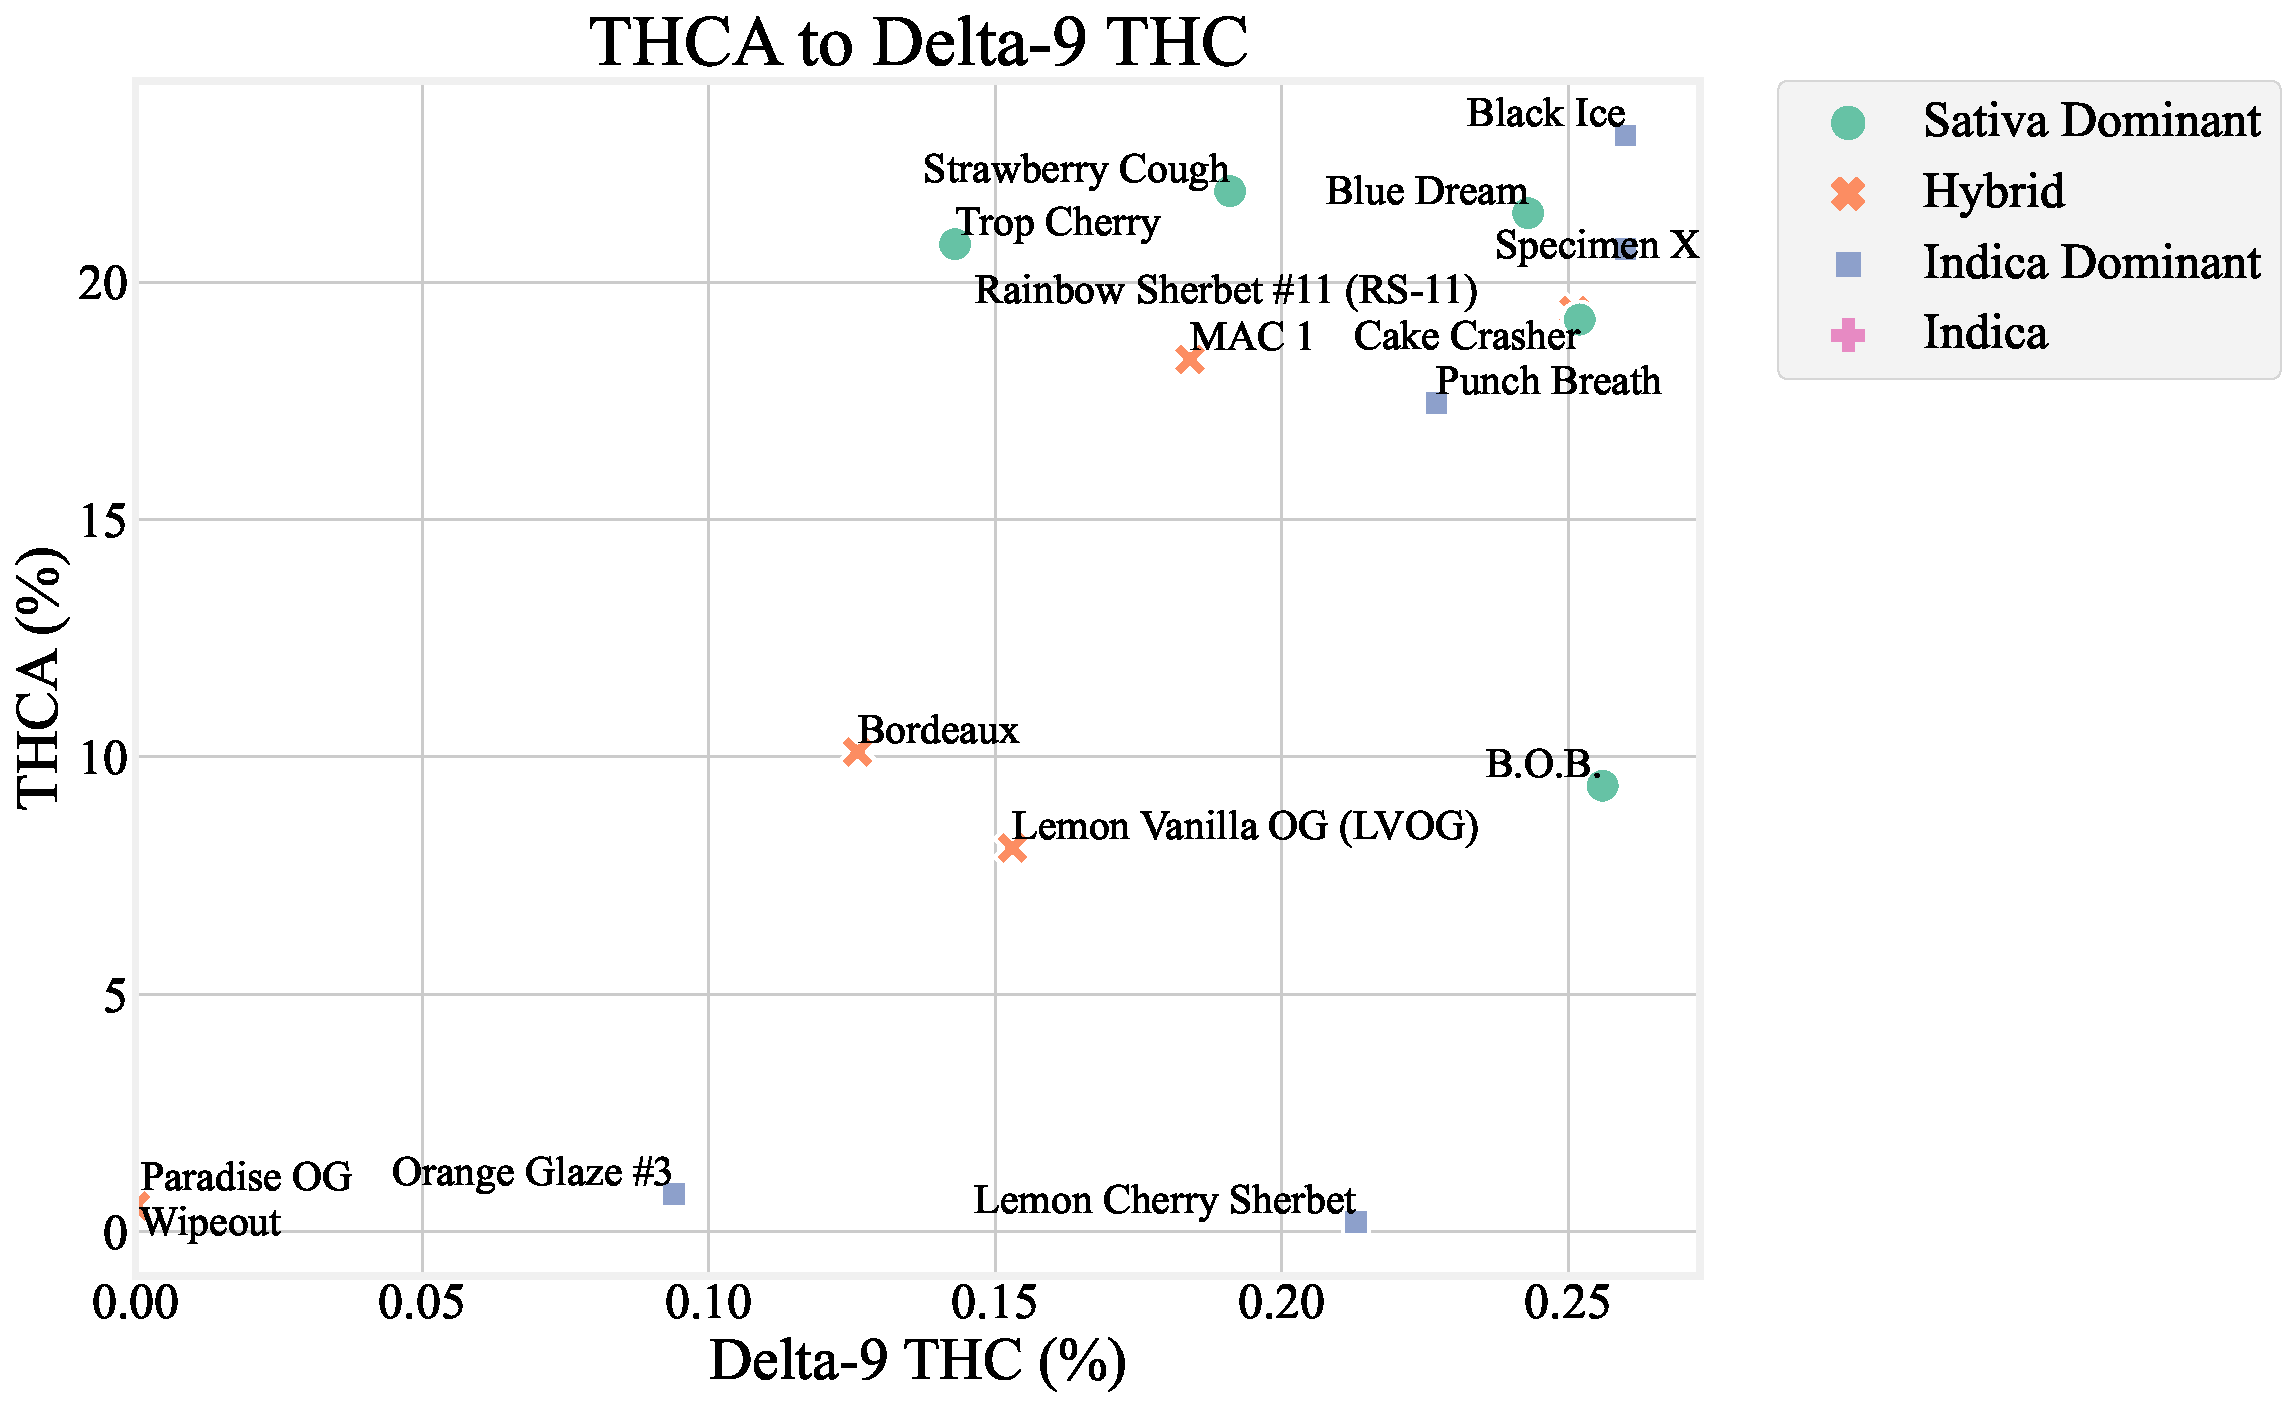
\includegraphics[width=\linewidth]{figures/thca-to-delta-9-thc.pdf}

\vspace{2\baselineskip}

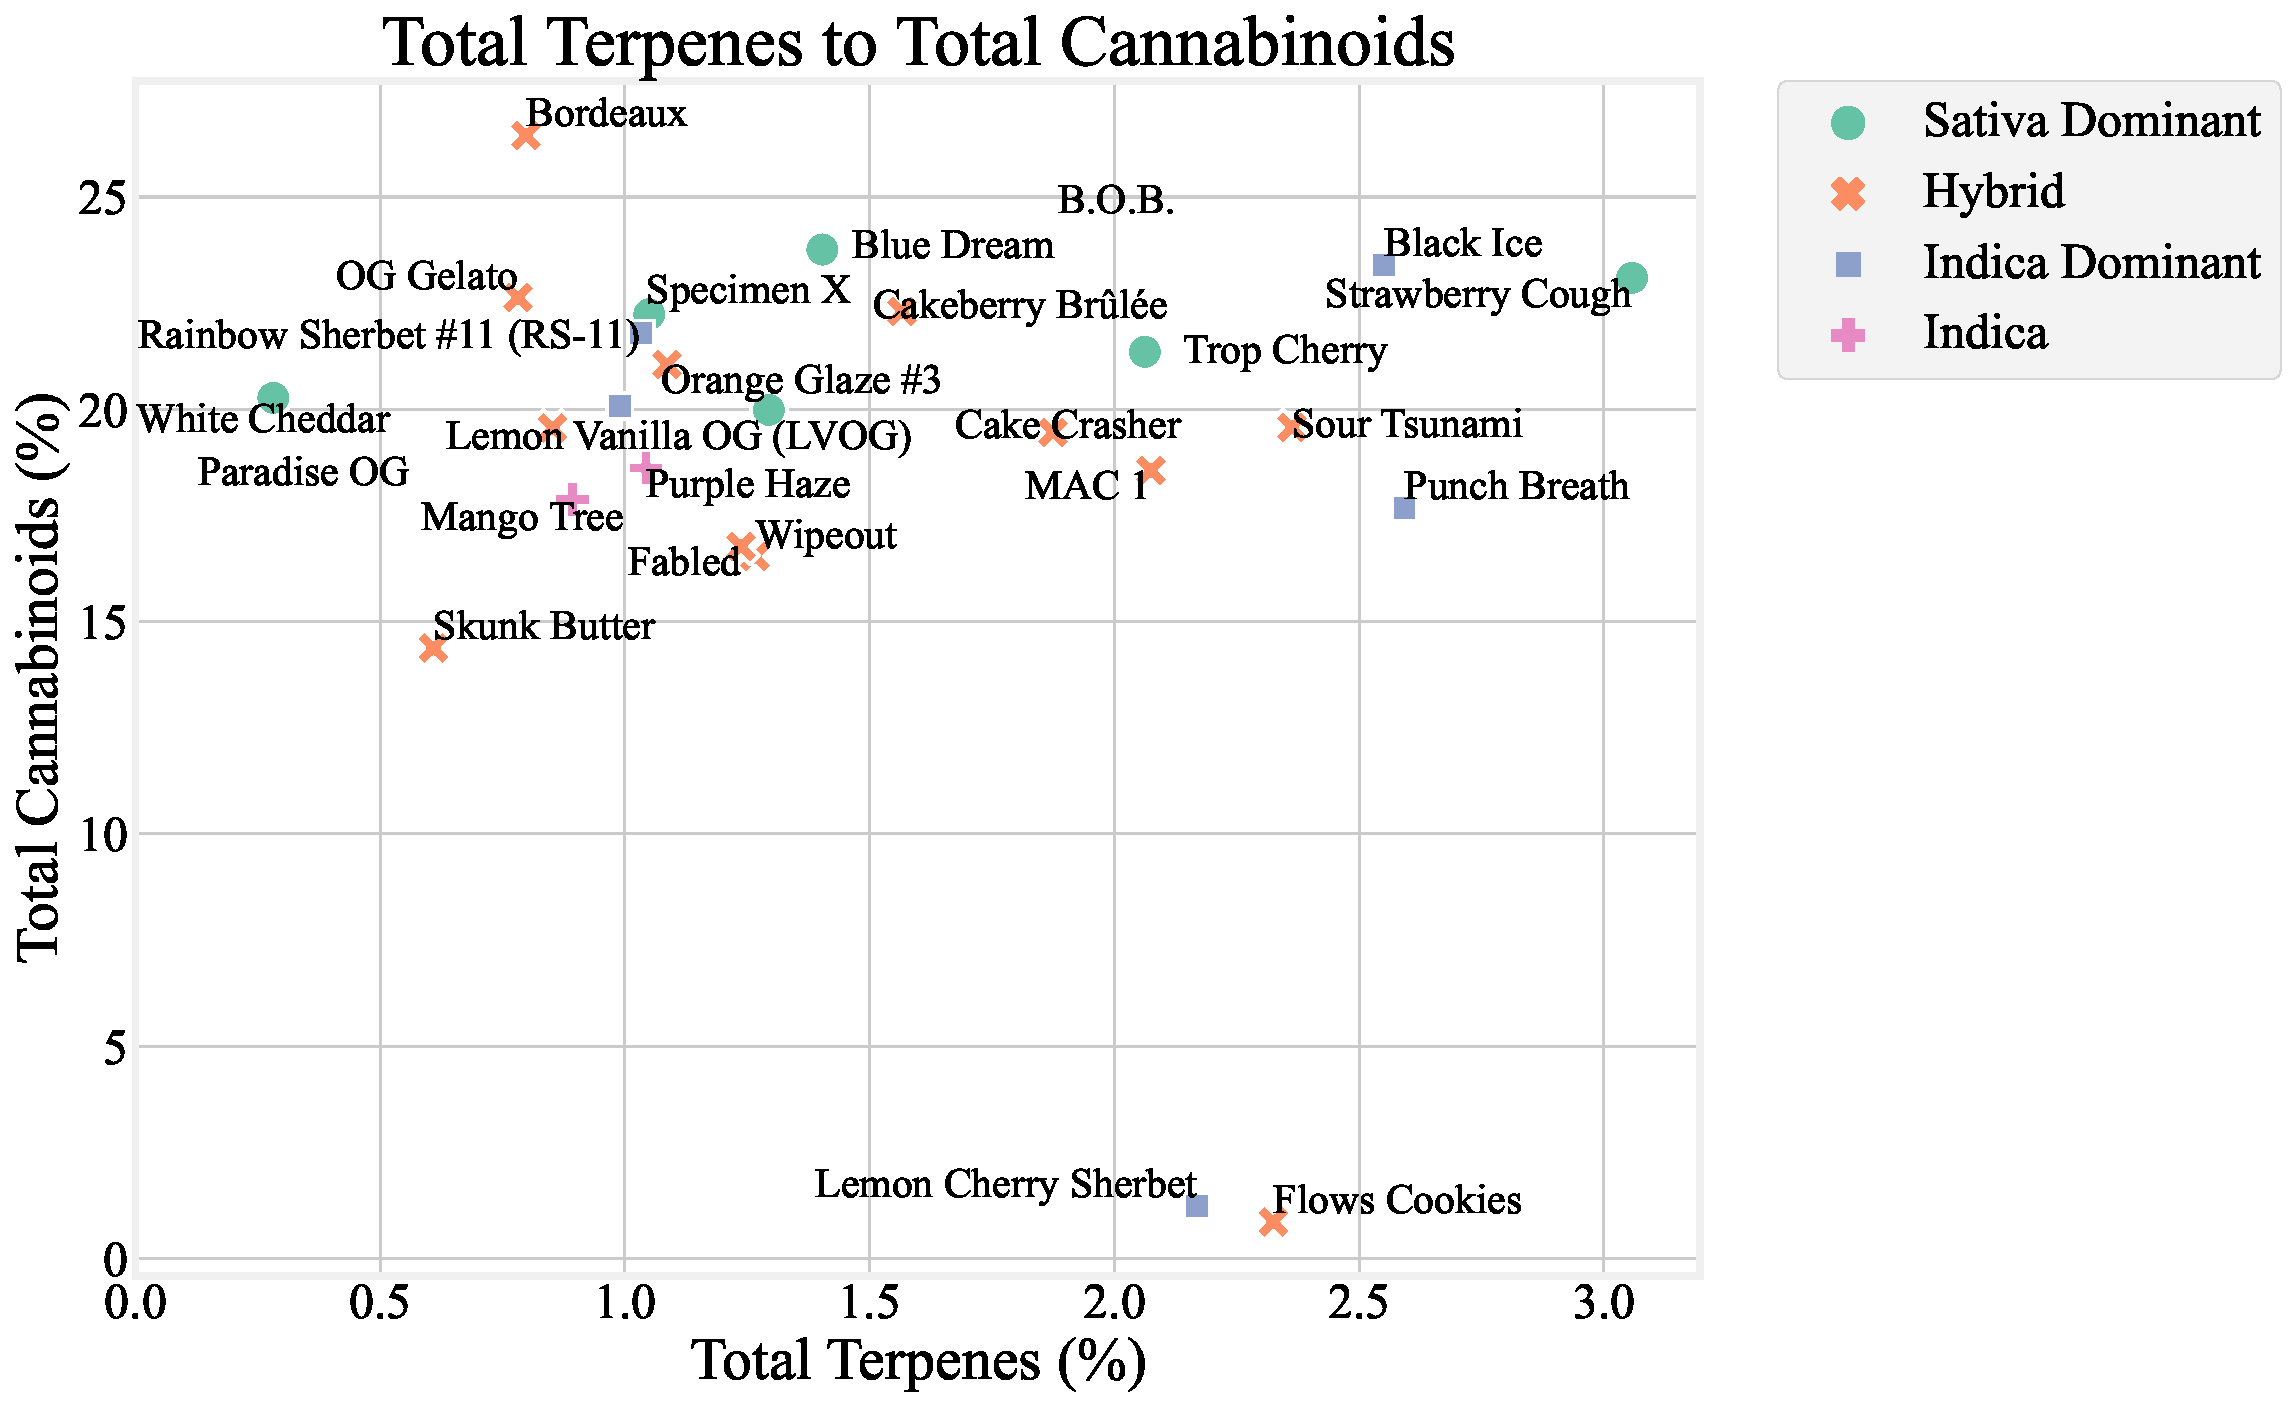
\includegraphics[width=\linewidth]{figures/sum-of-cannabinoids-to-sum-of-terpenes.pdf}

\vspace{2\baselineskip}

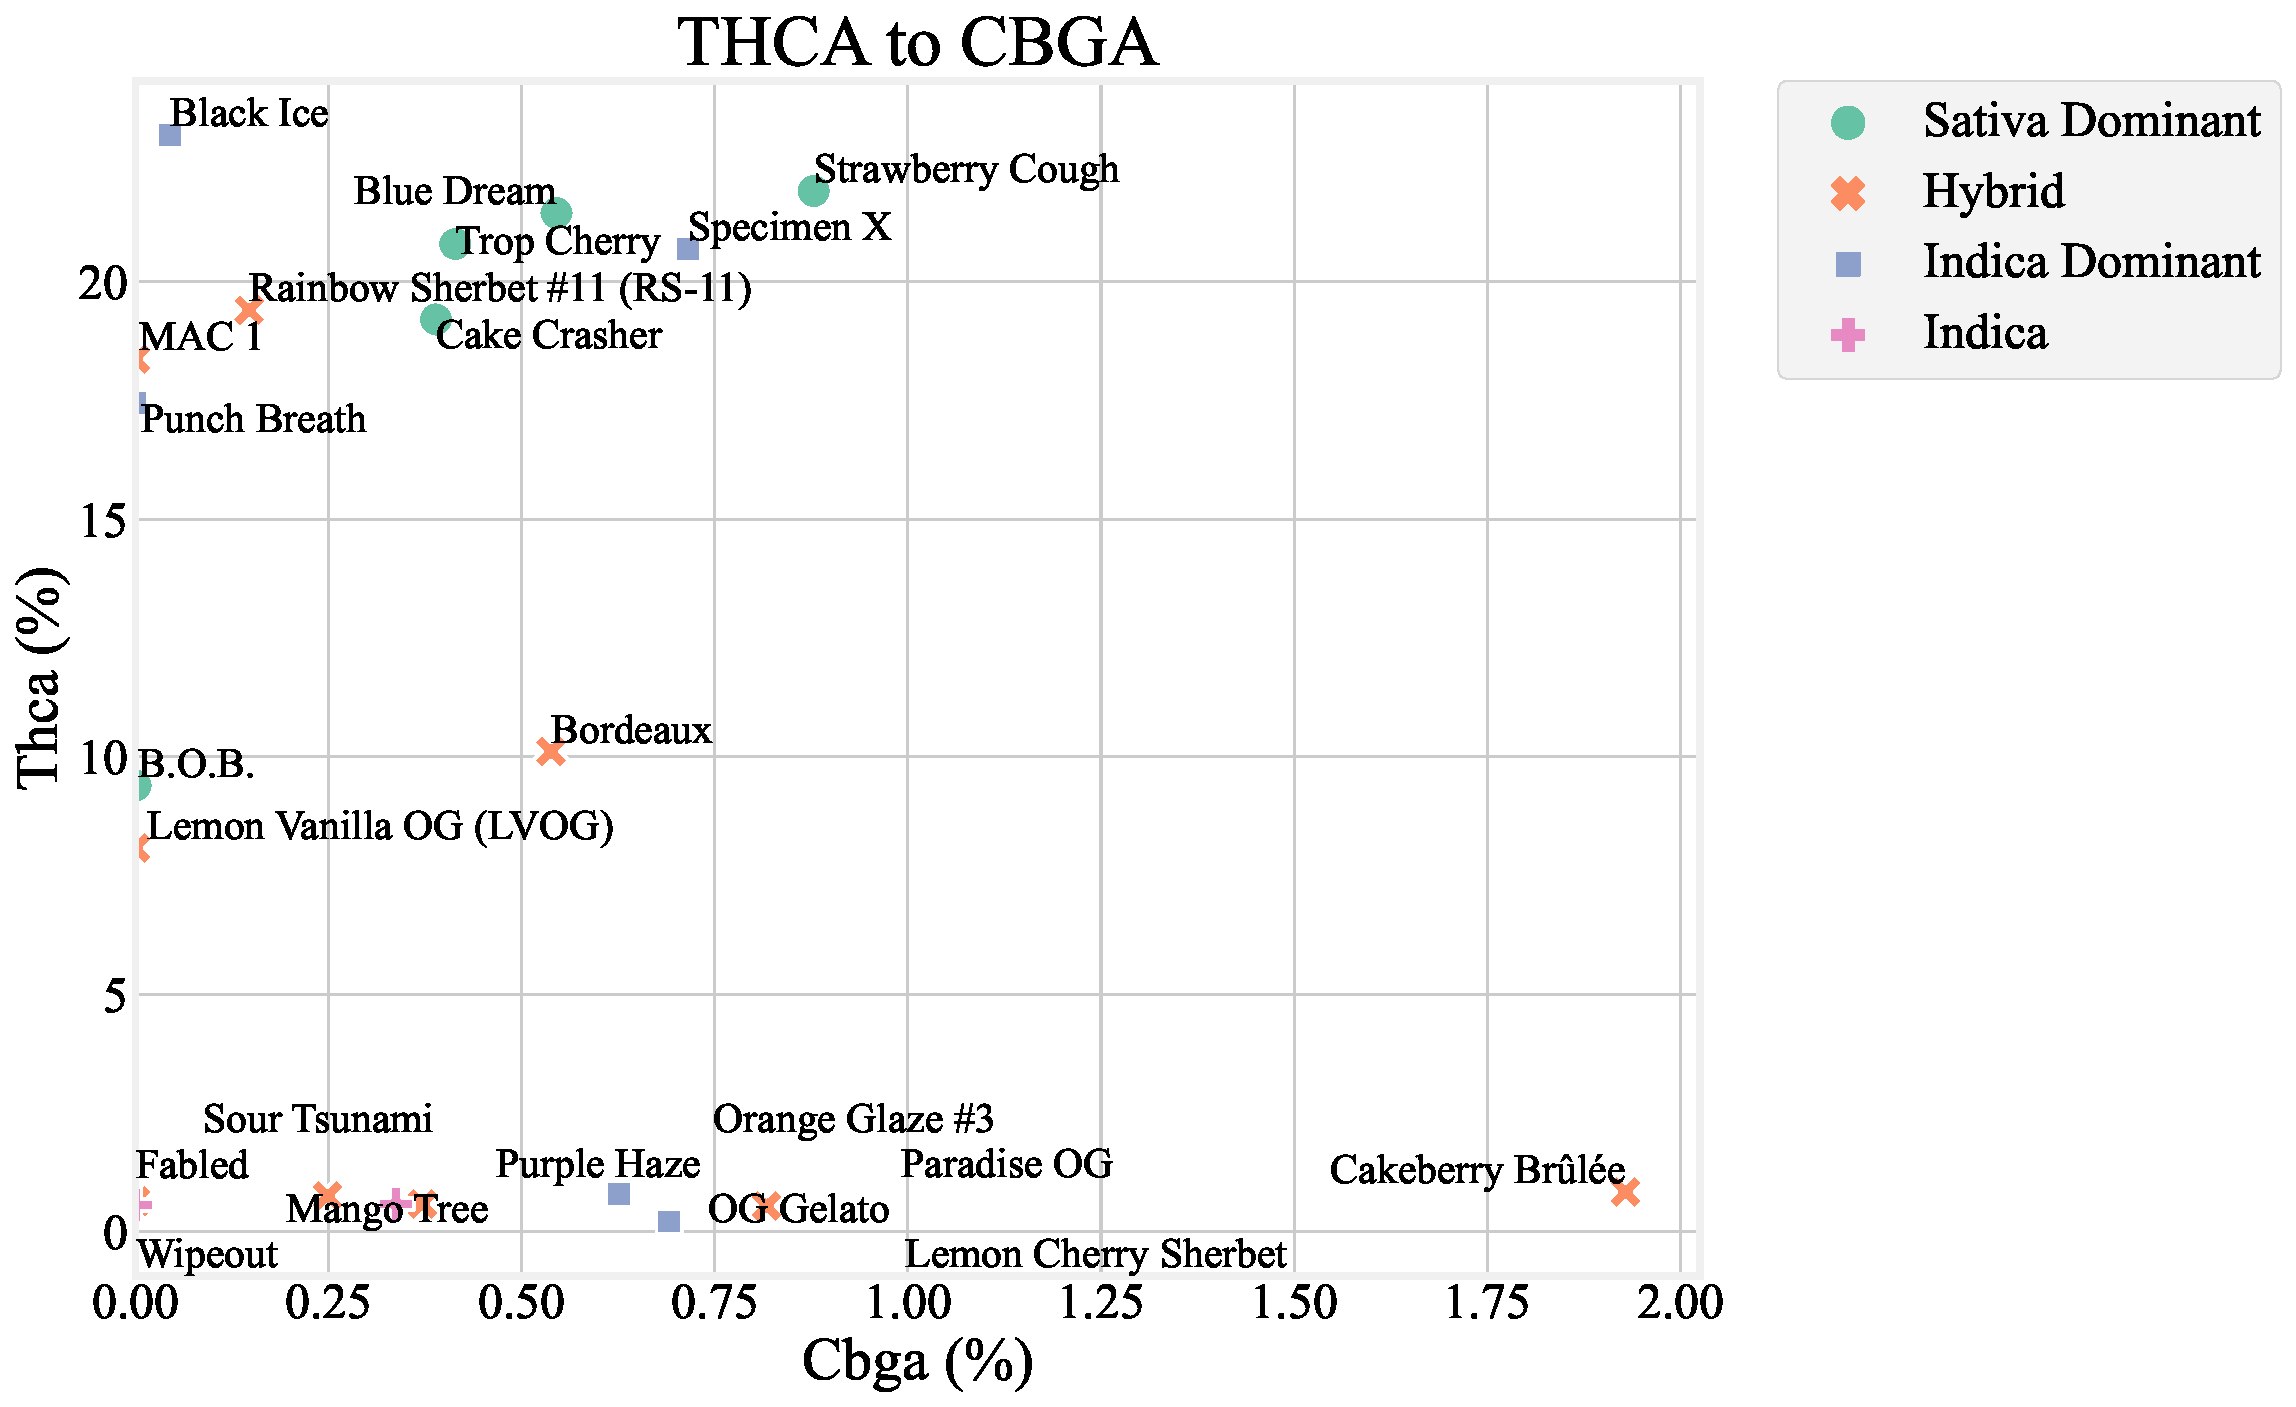
\includegraphics[width=\linewidth]{figures/thca-to-cbga.pdf}

\vspace{2\baselineskip}

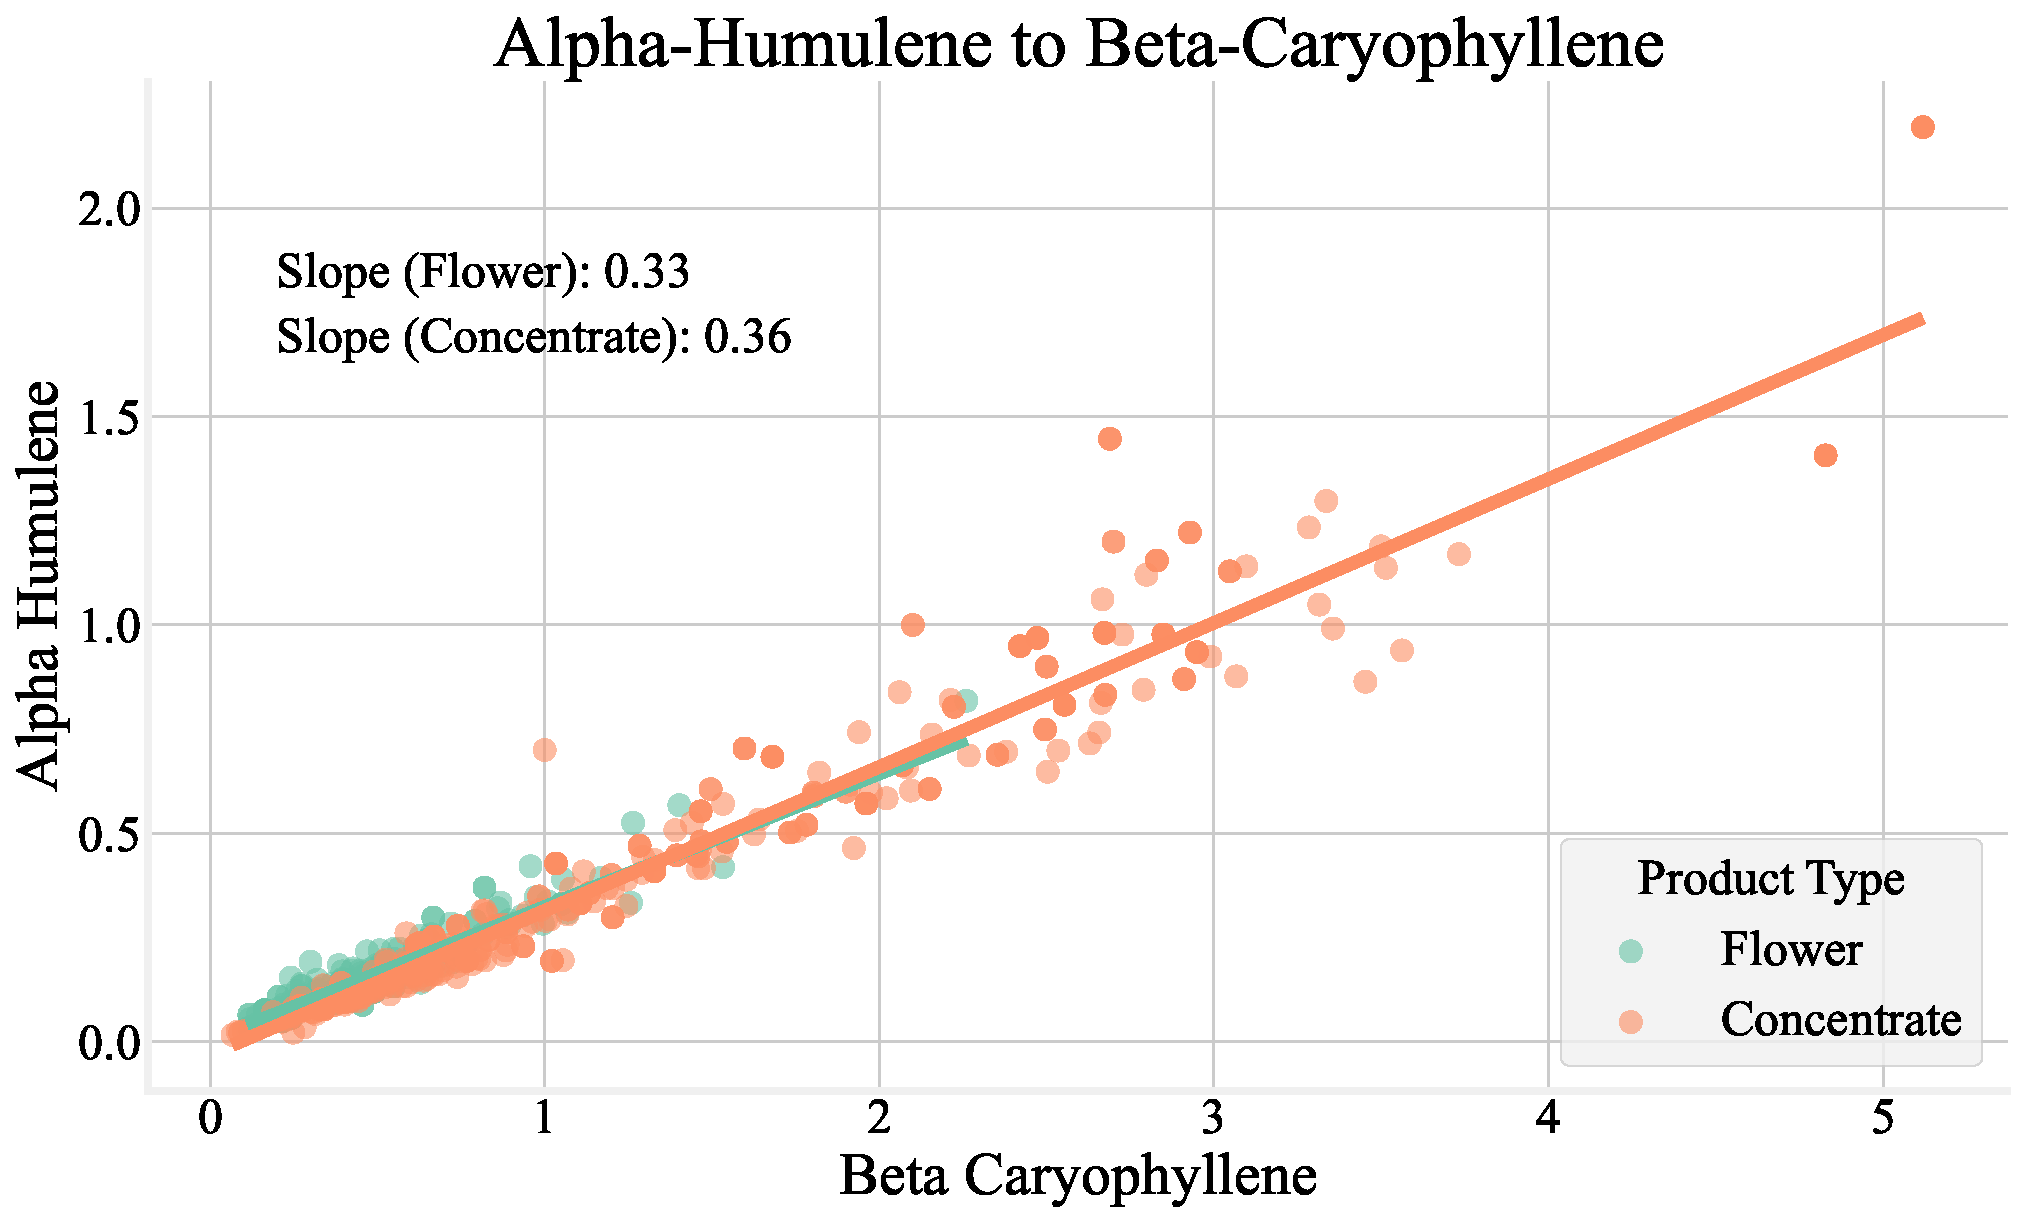
\includegraphics[width=\linewidth]{figures/alpha-humulene-to-beta-caryophyllene.pdf}

\vspace{2\baselineskip}

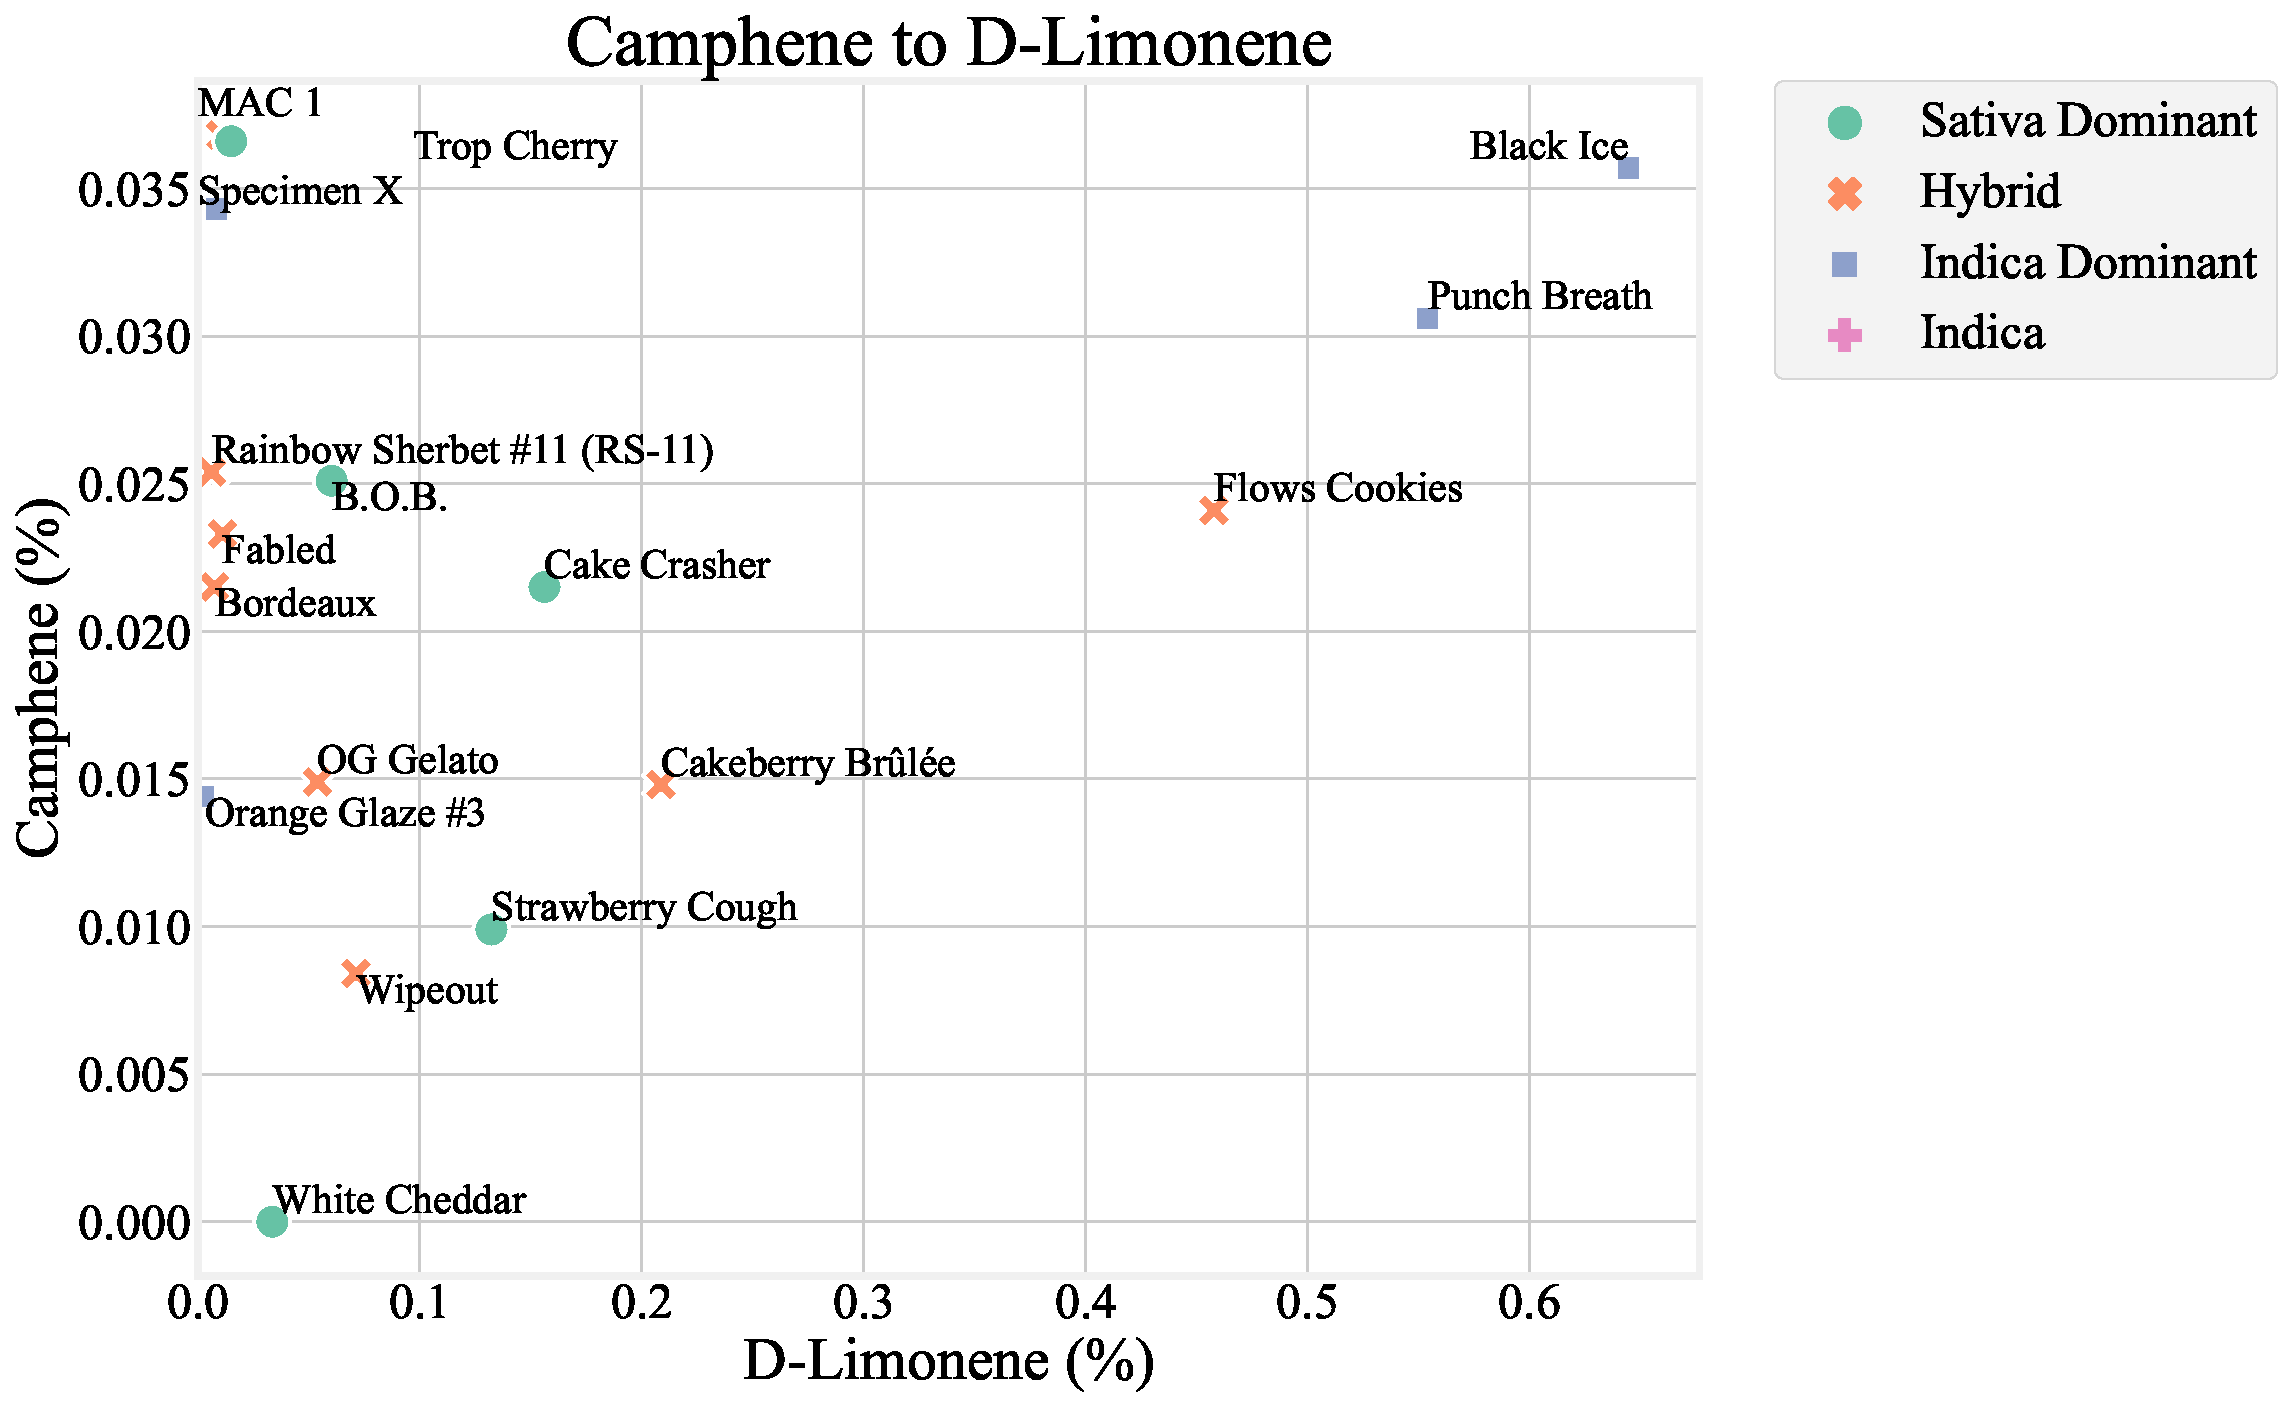
\includegraphics[width=\linewidth]{figures/camphene-to-d-limonene.pdf}

\vspace{2\baselineskip}

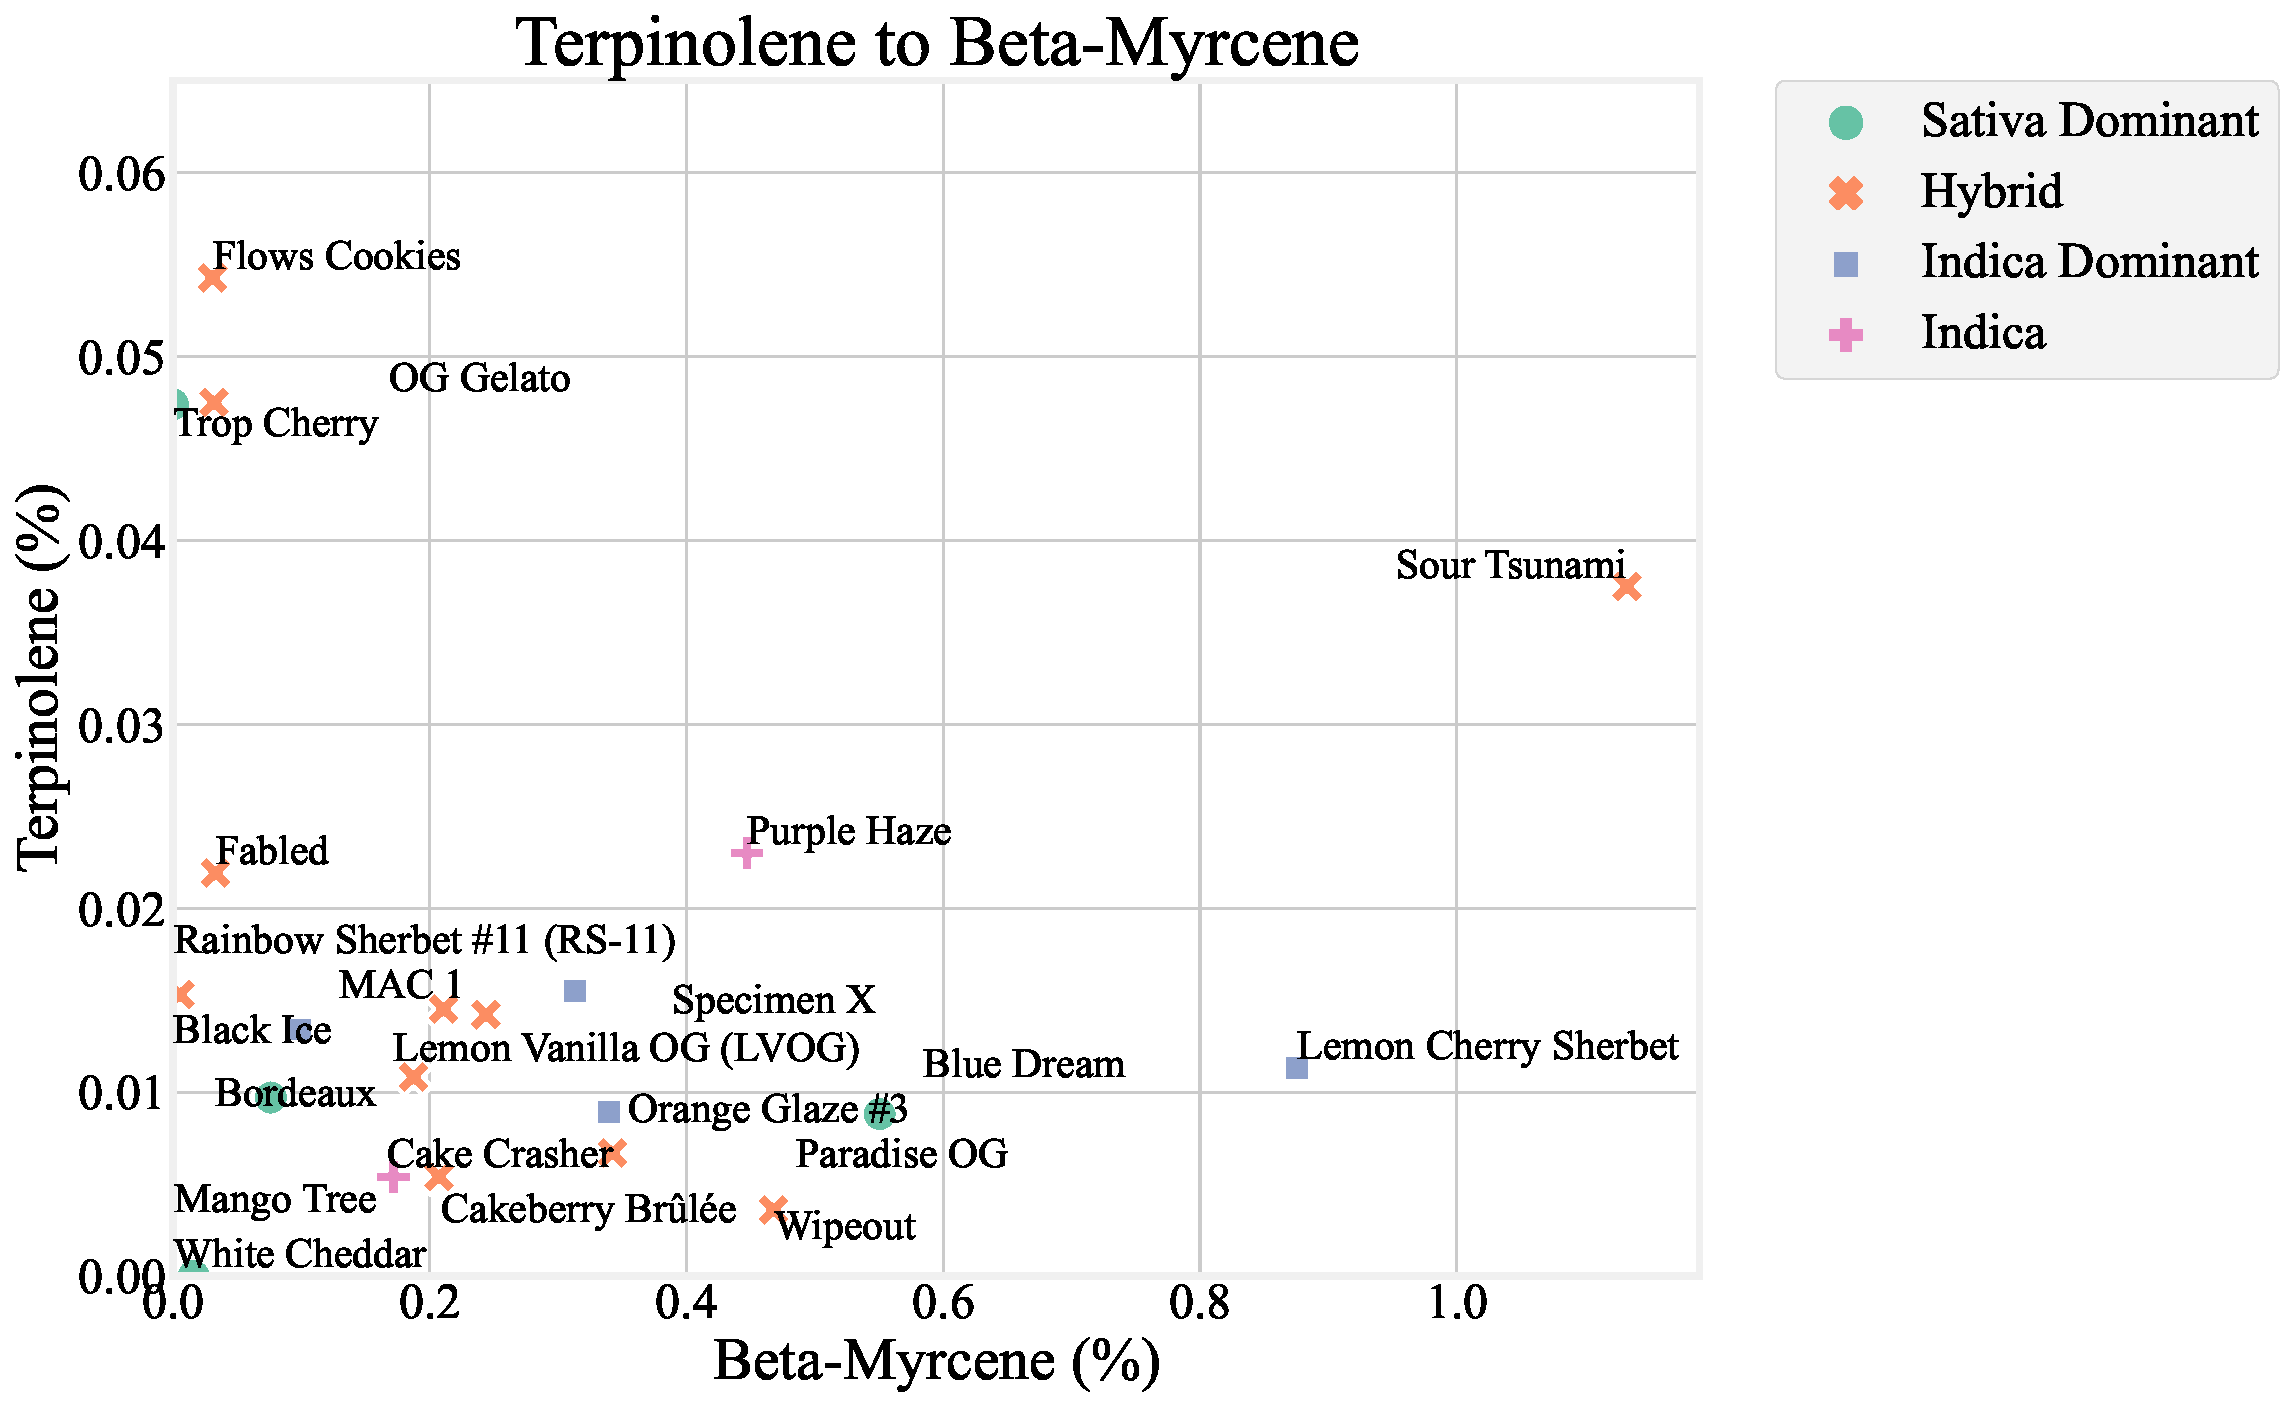
\includegraphics[width=\linewidth]{figures/terpinolene-to-beta-myrcene.pdf}

\vspace{2\baselineskip}

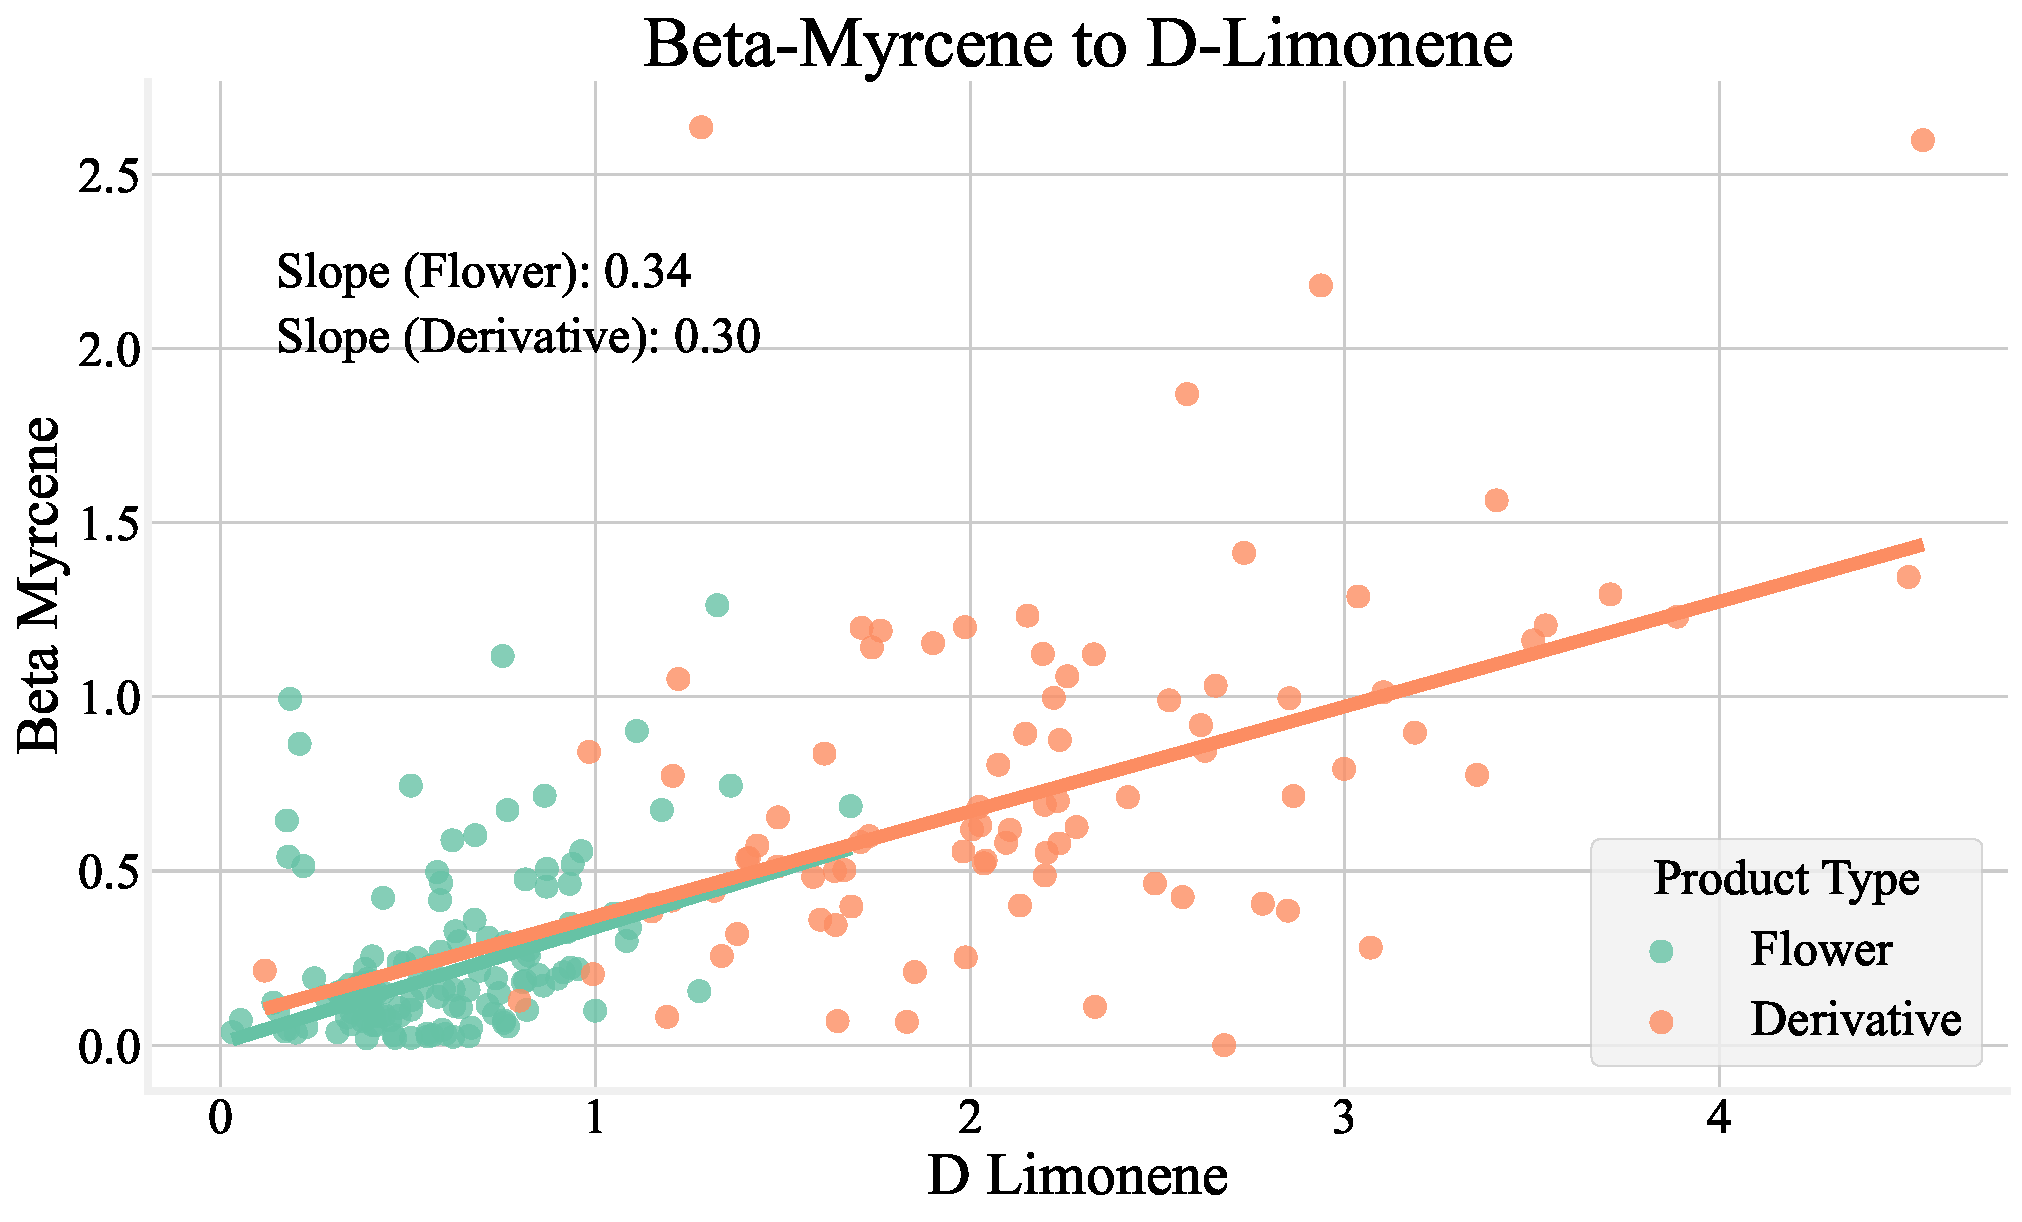
\includegraphics[width=\linewidth]{figures/beta-myrcene-to-d-limonene.pdf}

\vspace{2\baselineskip}

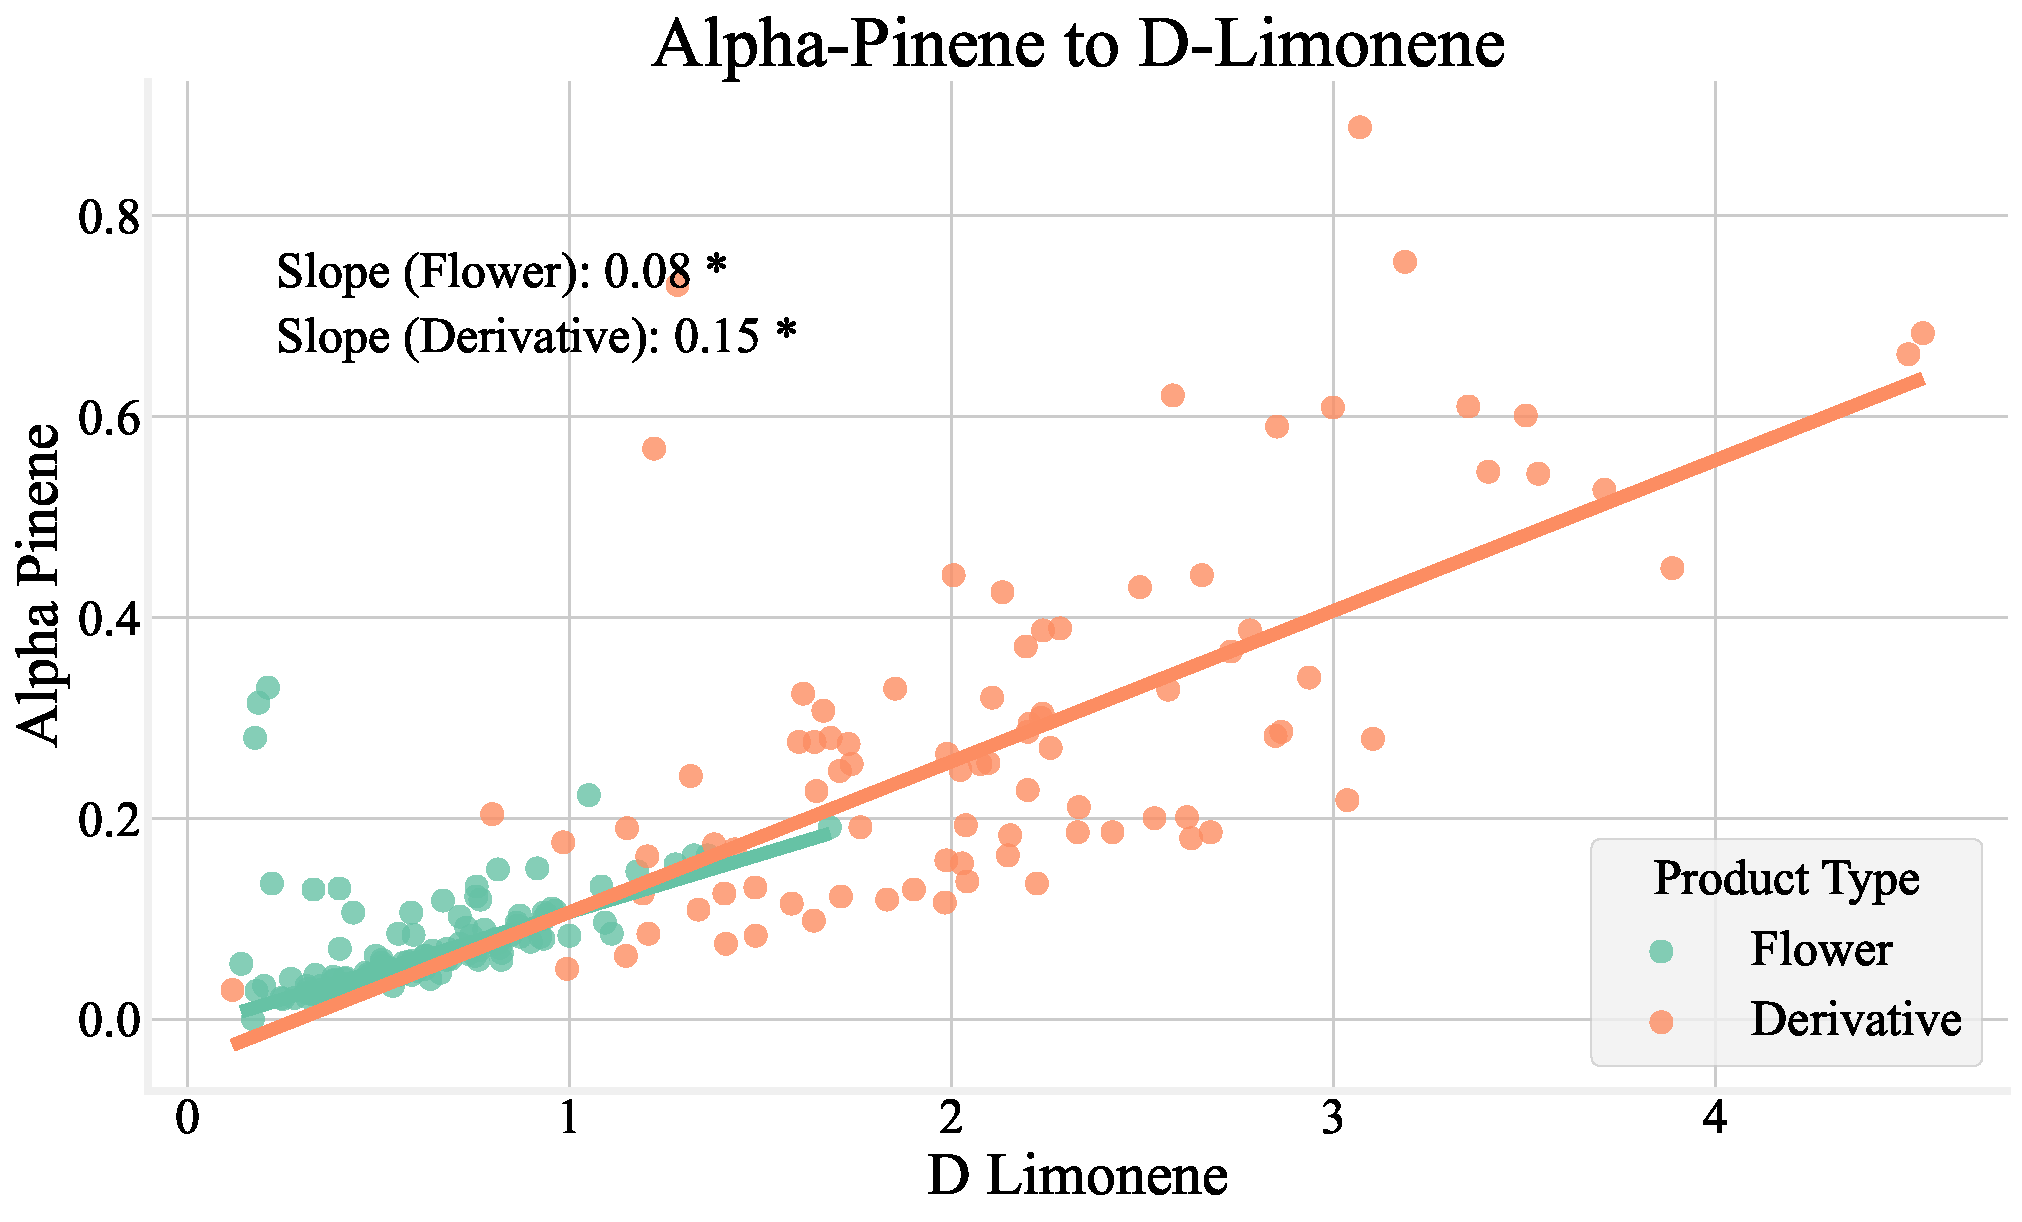
\includegraphics[width=\linewidth]{figures/alpha-pinene-to-d-limonene.pdf}

\vspace{2\baselineskip}

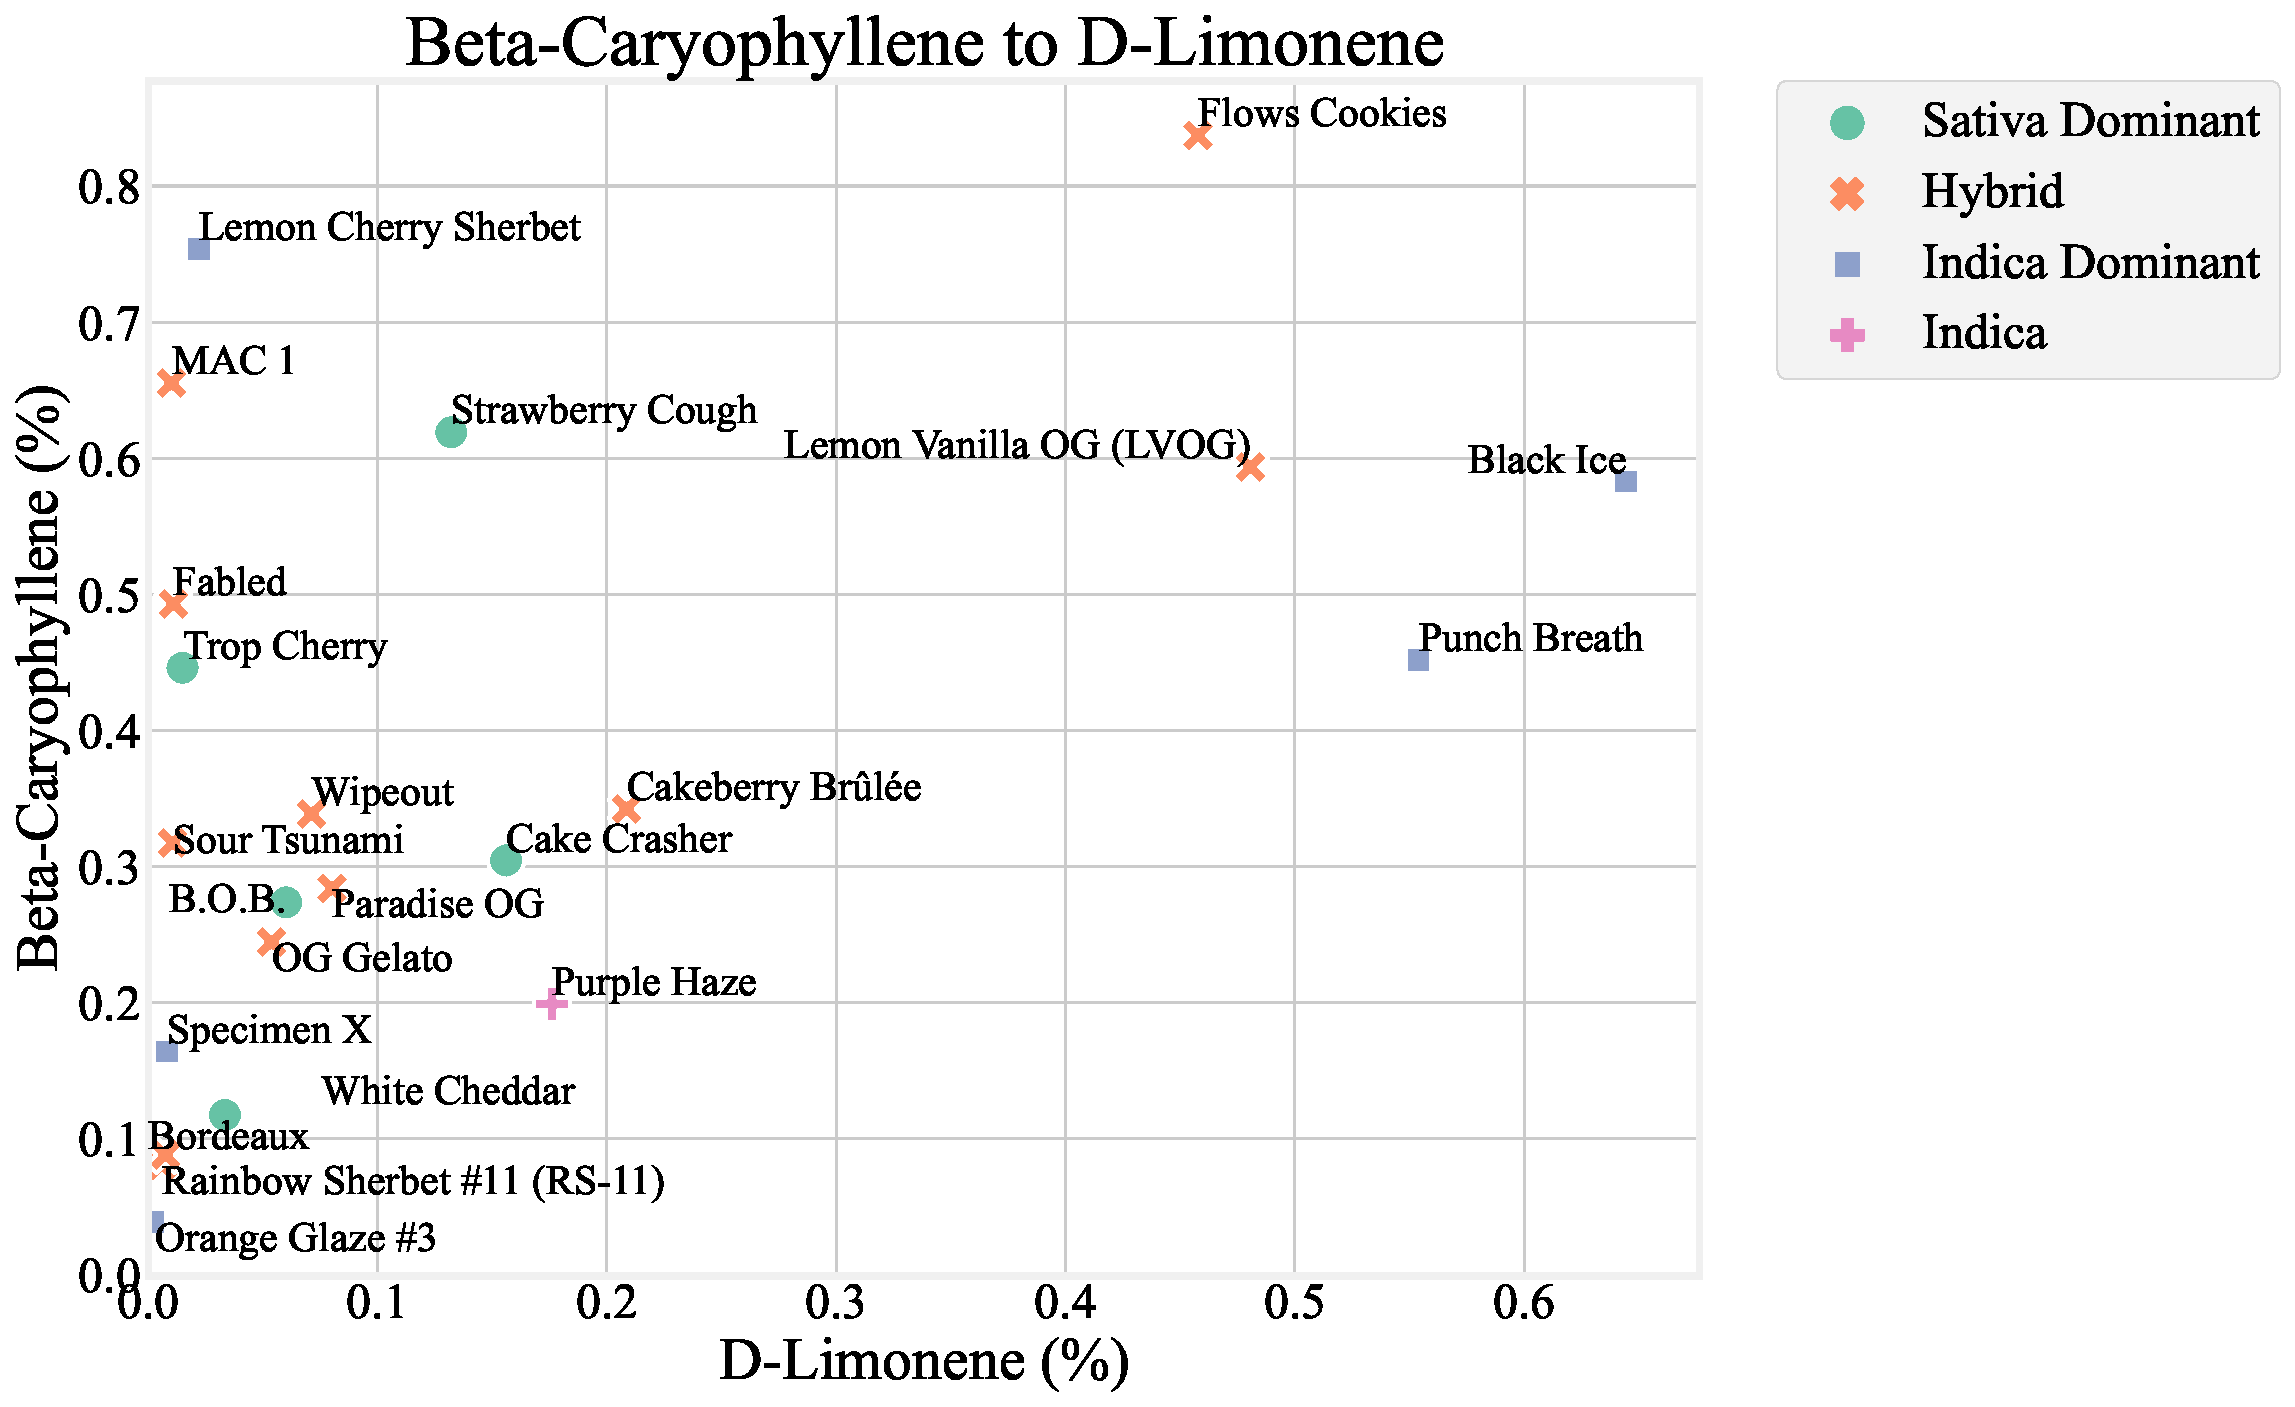
\includegraphics[width=\linewidth]{figures/beta-caryophyllene-to-d-limonene.pdf}

\vspace{2\baselineskip}

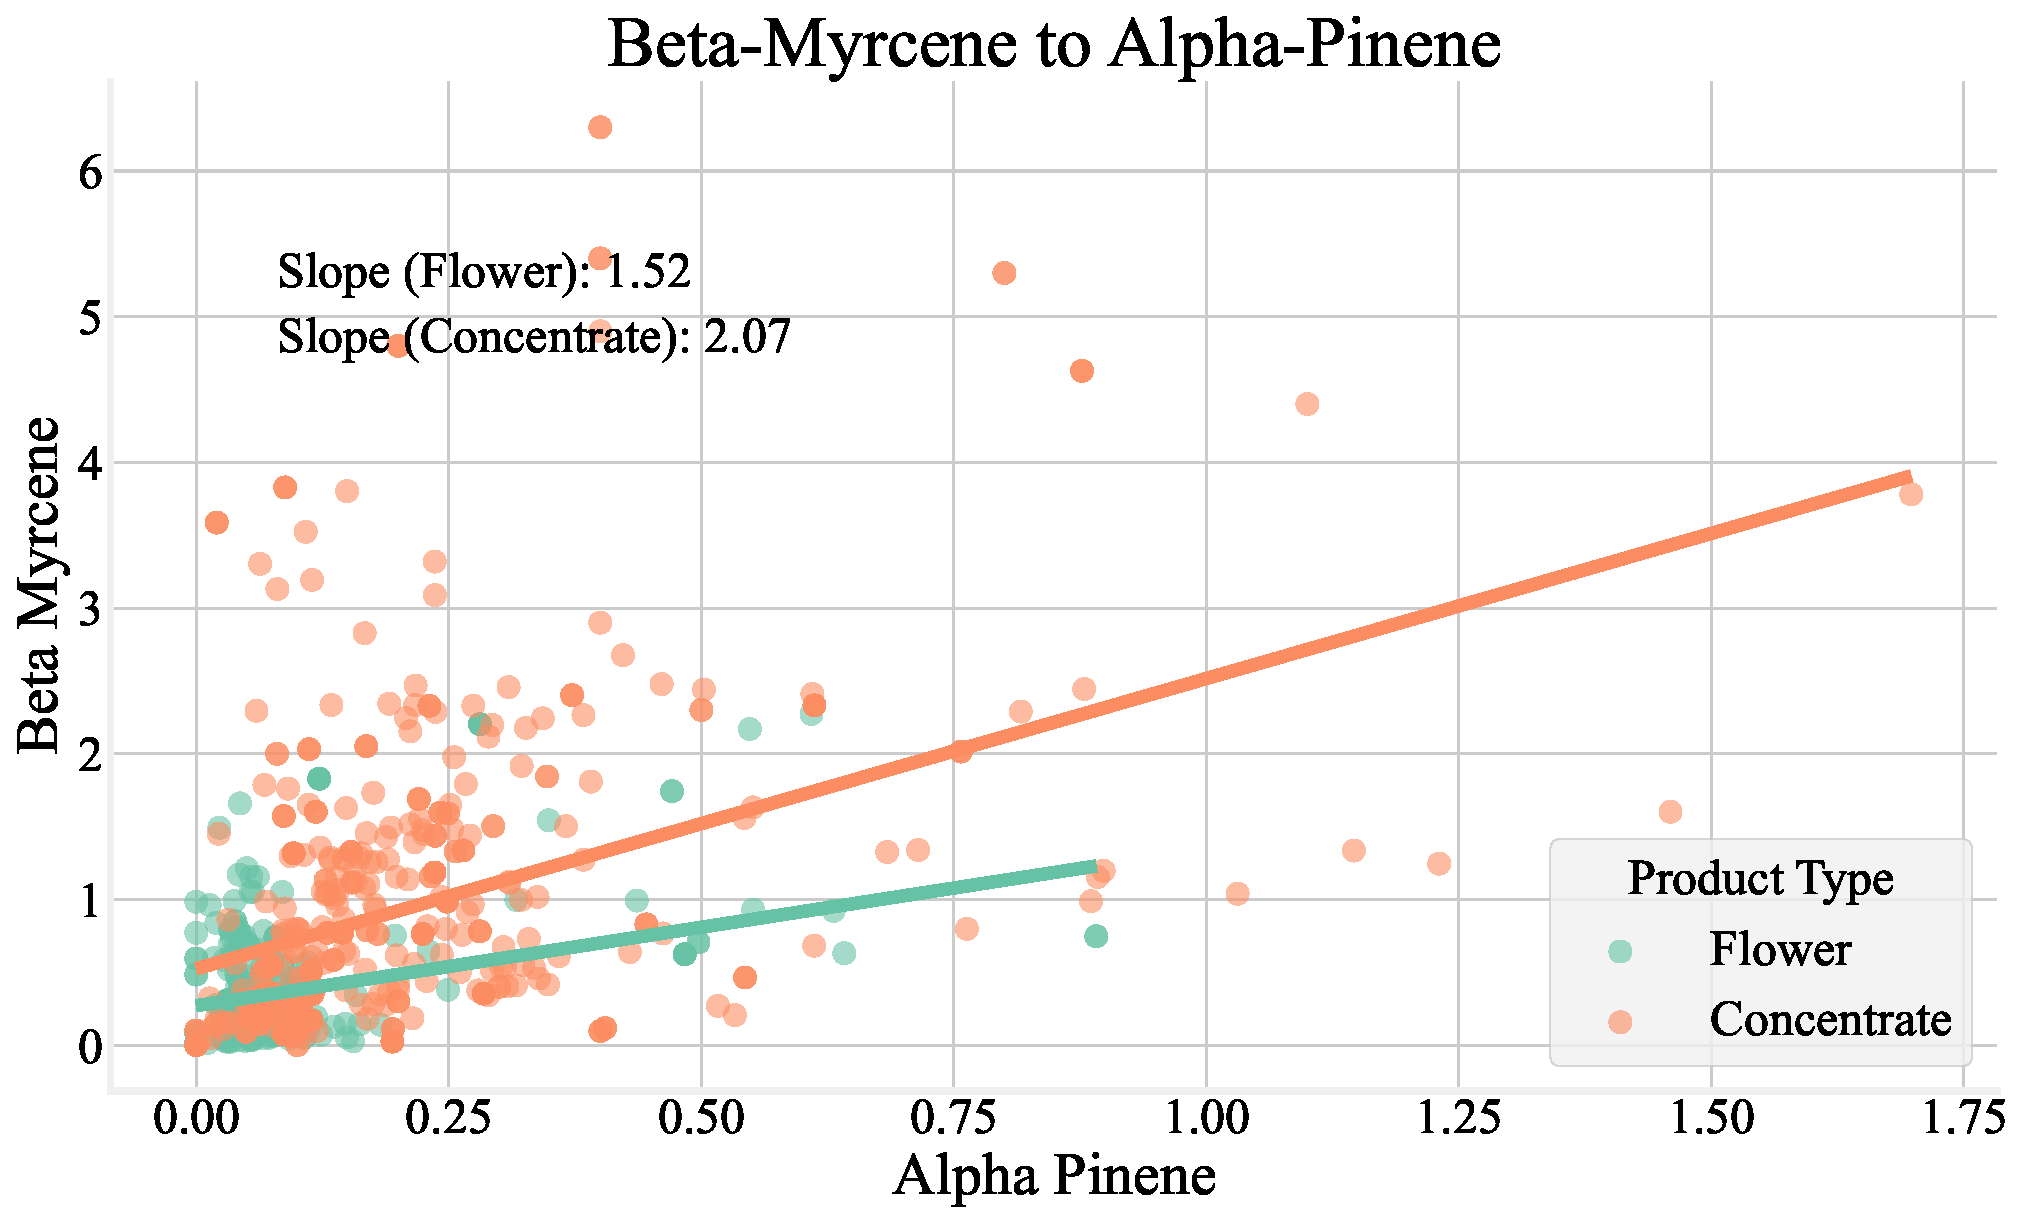
\includegraphics[width=\linewidth]{figures/beta-myrcene-to-alpha-pinene.pdf}

\end{multicols}

\vspace{2\baselineskip}

% PCA
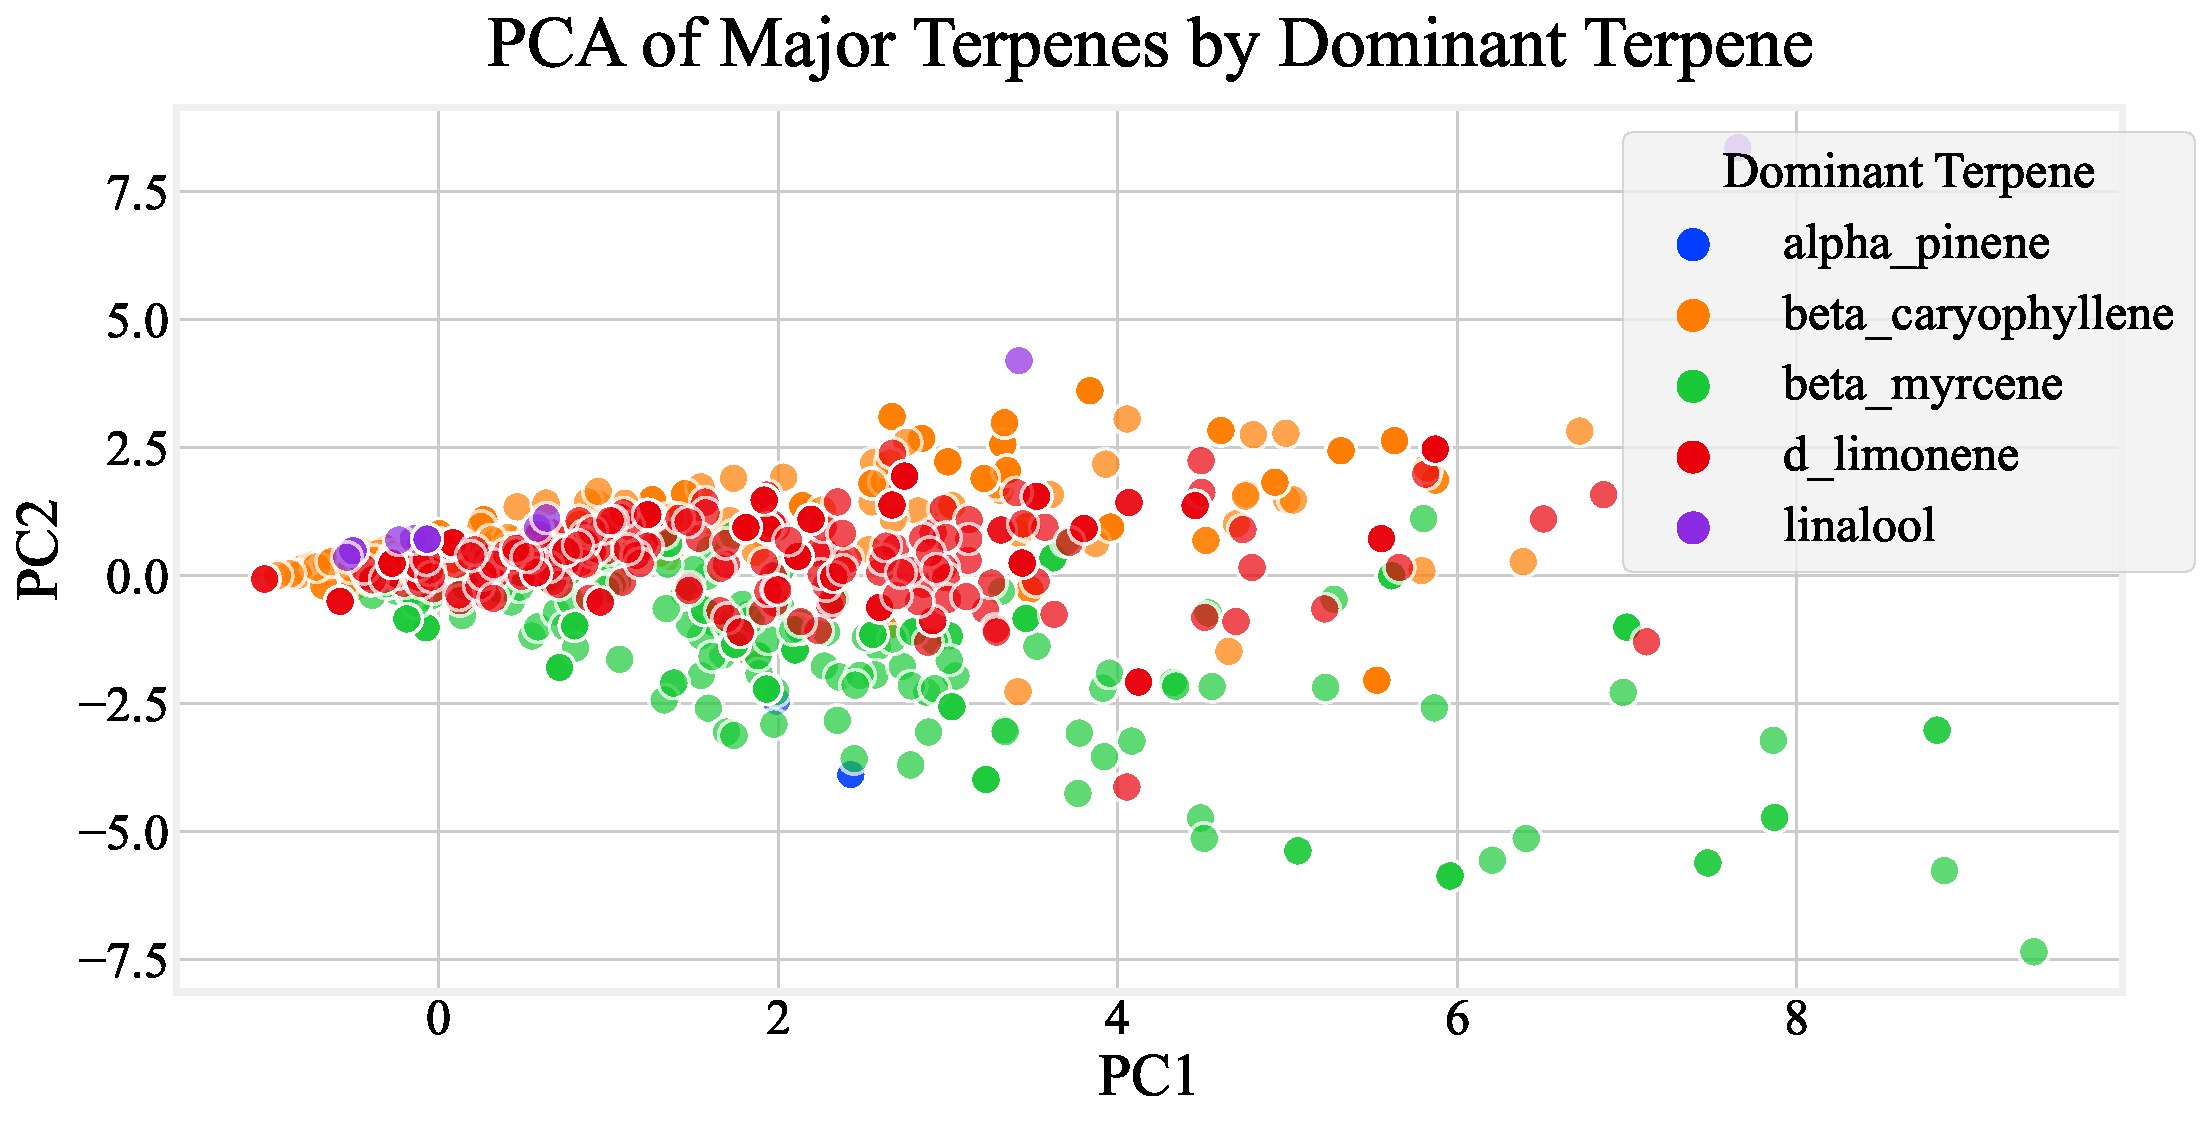
\includegraphics[width=\linewidth]{figures/pca-dominant-terpenes.pdf}


%---------------------------------%
% References
%---------------------------------%
%\newpage
%\nocite{*}
%\bibliography{references}
\thispagestyle{regular}

%---------------------------------%
% End of the Body
%---------------------------------%
\thispagestyle{regular}
\end{document}
